
%%\documentclass[12pt,oneside]{article}

\documentclass[smallcondensed]{svjour3}
%\providecommand{\event}{Journal TBD}
%\providecommand{\publicationstatus}{ } %% TBD - fill in any footer
%%\documentclass[12pt,oneside]{llncs}

%% Language %%%%%%%%%%%%%%%%%%%%%%%%%%%%%%%%%%%%%%%%%%%%%%%%%
\usepackage{hyperref}   %% sets hyperlinks within a pdf
\usepackage{graphicx}
\usepackage{epstopdf}
\usepackage{parskip}
\usepackage{enumitem}
\usepackage{wrapfig}
\usepackage{subcaption}
\usepackage{caption}
\usepackage{array}
\usepackage{color}
\usepackage{colortab}
\usepackage{xcolor}
\usepackage{tabularx}
\usepackage{pdfpages}

%%\usepackage{subcaption}

%%\usepackage{lmodern} %Type1-font for non-english texts and characters


%% Packages for Graphics & Figures %%%%%%%%%%%%%%%%%%%%%%%%%%
%\usepackage{graphicx} %%For loading graphic files
%\usepackage{subfig} %%Subfigures inside a figure
%\usepackage{tikz} %%Generate vector graphics from within LaTeX

%\usepackage{mathptmx} %% Times fonts, for math as well

%%\makeindex

%% The adjustment amounts depend on the font
%% -.5 for 12pt, -.875 for 10pt
%% FIXME: should these be set instead of adjusted?
%% Use these with lncls?
%\addtolength{\oddsidemargin}{-.5in}
%\addtolength{\evensidemargin}{-.5in}
%\addtolength{\textwidth}{1.0in}
%\addtolength{\topmargin}{-.5in}
%\addtolength{\textheight}{1.0in}

%\def\titlerunning{SMTEVAL-2013}
%\def\authorrunning{Cok, Stump, Weber}

\newcommand{\tb}{\textbullet}
\newcommand{\tjark}[1]{\marginpar{\footnotesize{#1}}}
\newcommand{\tjarkx}[1]{\makebox[0pt][c]{\raisebox{0pt}[0pt][0pt]{\Large\textcolor{red}{${}^*$}}}\marginpar{\footnotesize{#1}}}

\newcommand{\cellbr}[2][c]{\begin{tabular}[#1]{@{}c@{}}#2\end{tabular}}

\journalname{Journal of Automated Reasoning}

\begin{document}
\title{The 2013 Evaluation of SMT-COMP and SMT-LIB}

%\author{
%David R. Cok \\ GrammaTech, Inc., USA \\ \email{dcok@grammatech.com} \\ 
%Aaron Stump \\ University of Iowa, IA, USA \\ \email{aaron-stump@uiowa.edu} \\ 
%Tjark Weber \\ Uppsala University, Sweden \\ \email{tjark.weber@it.uu.se} }

%% eptcs format
\author{
David R. Cok 
\and  
Aaron Stump
\and  
Tjark Weber
}

\institute{
David R. Cok  \at GrammaTech, Inc., USA \email{dcok@grammatech.com}
\and
Aaron Stump \at University of Iowa, IA, USA \email{aaron-stump@uiowa.edu}
\and
Tjark Weber \at Uppsala University, Sweden \email{tjark.weber@it.uu.se}
}
%% lncls format
%\author{David R. Cok \inst{1} \and \\ 
%Aaron Stump \inst{2} \and \\ 
%Tjark Weber \inst{3}  \\
%}
%
%\institute{GrammaTech, Inc., USA \email{dcok@grammatech.com} \and
%University of Iowa, IA, USA \email{aaron-stump@uiowa.edu} \and
%Uppsala University, Sweden, \email{tjark.weber@it.uu.se}
%}


\date{\today}
\maketitle
%\pagestyle{headings}
%\pagenumbering{arabic}
%\centerline{\today}

%\abstract{
\begin{abstract}
After 8 years of SMT Competitions, the SMT Steering Committee decided,
for 2013, to sponsor an evaluation of the status of SMT benchmarks and
solvers, rather than another competition.  This report summarizes the
results of the evaluation, conducted by the authors.  The key
observations are that (1)~the competition results are quite sensitive
to randomness and (2)~the most significant need for the future is
assessment and improvement of benchmarks in the light of SMT
applications.  The evaluation also measured competitiveness of
solvers, general coverage of solvers, logics, and benchmarks, and
degree of repeatability of measurements and competitions.
\end{abstract}


\section{Introduction}

\subsection{The Competition history and goals}
From 2005 through 2012 (and coming again in 2014), the SMT community
sponsored an annual competition among SMT solvers
(cf.\ Fig.~\ref{Fig:history}).  The purpose of the competition is to
encourage advances in SMT solver implementations acting on benchmark
formulas of theoretical or practical interest.  Public competitions
are a well-known means of stimulating advancement in software tools.
For example, in automated reasoning, the SAT and CASC competitions for
propositional and first-order reasoning tools, respectively, have
spurred significant innovation in their fields~\cite{leberre+03,PSS02}.  Indeed, the SMT competition increased in
size each year: more benchmarks were added, new solver teams
participated, solver performance improved, and more logic divisions were defined.

The particular goals of SMT-COMP include the following~\cite{smtcompweb}:
\begin{itemize}[noitemsep]
\item enable research on SMT solvers by benchmarking and comparing performance;
\item promote a standard format for SMT problems (SMT-LIB v2~\cite{BarST-SMT-10});
\item collect additional benchmarks;
\item identify and develop new theories and logics for SMT, encouraging their inclusion in SMT solvers;
\item introduce SMT users and implementors to each other;
\item provide a forum for SMT implementors to promote their SMT solvers and for SMT users to assess the comparative performance of solvers; and
\item encourage the development of industrial-strength solvers for wide-spread use.
\end{itemize}

\begin{figure}
\centering
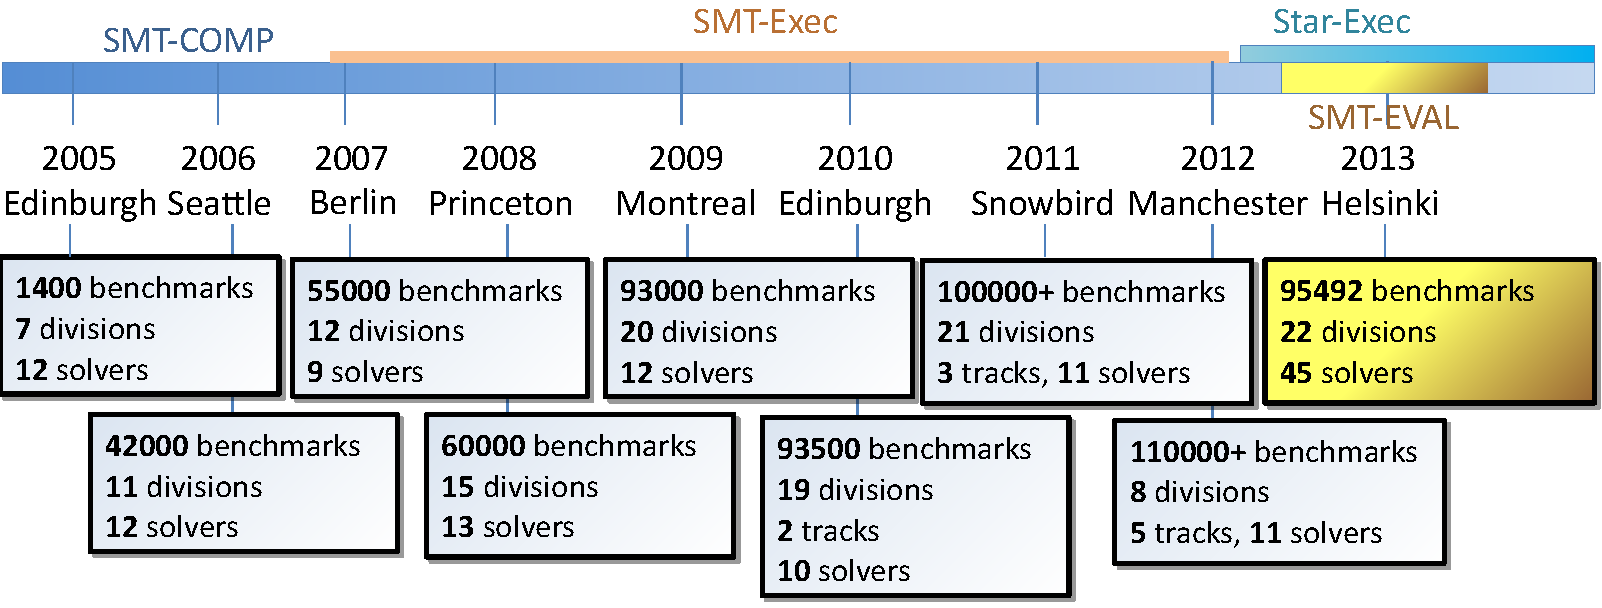
\includegraphics[width=\textwidth]{SMTCOMP-History}
\caption{SMT-COMP history}
\label{Fig:history}
\end{figure}

\subsection{Concerns prompting an evaluation}

In 2013, the SMT Steering Committee decided to take a collective breath and sponsor an evaluation of the current state of the art, without the pressure of a competition. In particular, the implementation teams found that preparing for a competition required considerable engineering work that detracted from other goals. On the one hand, the engineering work is necessary for users to use the tools as off-the-shelf applications. But holding the competition every year was causing some otherwise highly involved teams to withdraw. Thus there was a collective desire to pause the competition cycle for a year.

Second, there was a desire to evaluate the state of the SMT community and the competition. The competition had become focused on details of performance on a particular set of benchmarks for particular logics and there was a feeling that its overall results had become somewhat predictable. An evaluation of progress of the SMT community was desired, with a consideration of other metrics and goals, not just winning narrowly focused competitions.
 
And third, for many years the competition had relied on the SMT-Exec computational infrastructure~\cite{springerlink:10.1007/s10817-012-9246-5}.  A new infrastructure, Star-Exec~\cite{StuST-IJCAR-14,webStarExec} had been funded by the NSF and developed at the University of Iowa, but had not yet been tried out in earnest.  In fact, a goal in~2012 had been to use Star-Exec for SMT-COMP~2012; however, Star-Exec was not sufficiently operational and the competition had to revert to SMT-Exec.  It was anticipated that an evaluation in 2013, with less deadline pressure, would enable using Star-Exec on a shake-down cruise prior to a competition in 2014 at the Federated Logic Conference~(FLoC) Olympic Games~\cite{webOlympicGames}.

\subsection{Evaluation topics}

The SMT Steering Committee appointed a team of evaluators (the authors
of this report) to examine areas of interest. The evaluators, who are
not affiliated with any solver team, independently studied the
following topics:
\begin{itemize}[noitemsep]
\item continuity and turnover in SMT solver participation in past competitions (\ref{Solvers})
\item the performance of all historical and current solvers on the full set of benchmarks, measuring
\begin{itemize}[noitemsep]
\item the improvement in performance over time (\ref{Progress})
\item repeatability of performance measurements (\ref{Accuracy})
\item repeatability of competition results (\ref{CompetitionRepeatability})
\item competitiveness of solvers (\ref{Competitiveness})
\item parallel vs. sequential performance (\ref{parallel})
\end{itemize}
\item the usefulness of various logics
\begin{itemize}[noitemsep]
\item characteristics of existing logics (\ref{Lattice})
\item which logics are implemented by solvers (\ref{Coverage})
\item which logics are particularly relevant to application areas (\ref{Applications})
\end{itemize}
\item the state of existing benchmarks
\begin{itemize}[noitemsep]
\item the range of computational difficulty of the benchmarks (\ref{Benchmarks})
\item the degree to which benchmarks discriminate among solvers (\ref{Benchmarks})
\item which logics have support in benchmarks (\ref{Benchmarks})
\end{itemize}
\end{itemize}


\section{Evaluation tools}

\subsection{SMT-LIB benchmarks}

One goal of the SMT project since its inception has been collecting benchmarks by which to evaluate SMT solvers and to represent challenge problems in the field. The growth in the number of benchmarks available is shown in the graphics of Fig.~\ref{Fig:history}. All\footnote{One benchmark, added late, was not included in all of the data accumulation; hence some tables report 95\,491 benchmarks and some 95\,492.} of the benchmarks present in Star-Exec at the time of evaluation (95\,492 benchmarks) were used for the evaluation, including those with unknown status. Of course, in previous years only a subset of these were available, since new benchmarks were added from year to year. Also in 2012, some benchmarks were used in the competition that were not yet added into the SMT-LIB benchmark set and were not yet in StarExec at the time of the evaluation. The 2012 benchmark set also included some incremental benchmarks that were not used in this evaluation. Furthermore, the competition each year used a random selection of benchmarks (guided by a difficulty distribution). The fact that the set of benchmarks used in competitions was different each year muddied any year-to-year comparison of results. By using all available benchmarks in the evaluation, we intend that any comparative assessments across years or solvers be less susceptible to random choices (cf.~Section~\ref{CompetitionRepeatability}). The various kinds of benchmarks and their distribution across logics are discussed below in Section~\ref{Evaluations}.

\subsection{Solvers}

The SMT competitions required that participating solvers be publicly available Linux applications, and that they be available for any future experimenter to use on new experiments. Thus all historical solvers are still available. However, in 2010, the competition adopted the then new benchmark format, SMT-LIB~v2~\cite{BarST-SMT-10}. Thus solvers prior to 2010 do not run on the current benchmark set. The participating solvers are shown in Fig.~\ref{Fig:solvers}.

\begin{figure}
\centering
\begin{tabular}{|l|l|*{8}{c@{\hskip 10pt}}c|}
\hline
Solver & Affiliation & & \rotatebox[origin=c]{90}{2005} & \rotatebox[origin=c]{90}{2006} & \rotatebox[origin=c]{90}{2007} & \rotatebox[origin=c]{90}{2008} & \rotatebox[origin=c]{90}{2009} & \rotatebox[origin=c]{90}{2010} & \rotatebox[origin=c]{90}{2011} & \rotatebox[origin=c]{90}{2012} & \rotatebox[origin=c]{90}{2013} \\ \hline
Number participating & & &  11 & 11 & 9 & 13 & 12 & 10 & 13 & 13 & 9 \\ \hline
Abziz... & Cairo U. & & & & & & & & \textbullet\textbullet & +++ & \\
Boolector & JKU    & & & & & X & X & & + & + & \textbullet \\
CVC/CVCLite/CVC3 & NYU & & X & X & X & X & X & + & + & + & \\
CVC4 & NYU & & & & & & & + & + & + & \textbullet \\
MathSat-HeavyBV & Trento  & & & & & & & & & + & \\
MathSAT 3,4,5 & FBK       & & X & X & X & X & X & + & + & + & \textbullet \\
SMTInterpol & U. Freiburg & & & & & & & & + & + & \textbullet \\
SONOLAR & U. Bremen       & & & & & & & + & + & + & \textbullet \\
STP, simplifyingSTP, STP2 & U. Melbourne & & & X & & & X & + & + & + & \\
4Simp & U. Melbourne  & & & & & & & & & + & \\
Tiffany de Wintermontte & U. Melbourne  & & & & & & & & & + & \\
opensmt & U. Ligano  & & & & & X & X  & + & +  &  & \textbullet \\
veriT & UFRN & & & & &   & X  & + & +  &  & \textbullet \\
Z3 & MSR & & & & X & X  & &  & +  &  & \textbullet \\
AProVE NIA & RWTH Aachen & & & &  &   & &  + & +  &  &  \\
MiniSMT & U. Innsbruck & & & &  &   & &  + &   &  &  \textbullet \\
test\_pmathsat & FBK-IRST  & & & &  &   & &  + &   &  &   \\
barcelogic & UPC & &  X & X  & X  & X & X & & & &  \\ 
beaver & UC Berkeley & &   &   &   & X & X & & & &  \\ 
clsat & Washington U. & &   &   &   & X & X & & & &  \\ 
Sateen & U. Col-Boulder & &  X & X  & X  & X & X & & & &  \\ 
Spear & & &   &   & X  & X &  & & & &  \\ 
sword & U. Bremen & & &   & & X & X & & & &  \\ 
Yices & SRI & &  X & X  & X  & X & X & & & &  \\ 
alt-ergo & & &  &  &  & X & & & & &  \\ 
ArgoLib & & &  &  & X & & & & & &  \\ 
Fx7 & & &  &  & X & & & & & &  \\ 
Ario & & & X & X & & & & & & &  \\ 
ExtSat & & &  & X & & & & & & &  \\ 
HTP & & & X & X & & & & & & &  \\
Jat & & &  & X & & & & & & &  \\ 
NuSMV & & &  & X & & & & & & &  \\ 
Sammy & & & X & & & & & & & &  \\ 
SBT & & & X & & & & & & & &  \\ 
Simplics & & & X & & & & & & & &  \\ 
SVC & & & X & & & & & & & &  \\ \hline


\end{tabular}

\caption{Solvers used in each year of SMT-COMP and SMT-EVAL. Solvers prior to 2010 (marked by~X) do not support SMT-LIB~v2 and were not used for SMT-EVAL. Boxes marked with a~\textbullet{} symbol identify solvers that are new for the evaluation; all solvers since 2010 (marked with~+ or~\textbullet{} symbols) were used for the evaluation.}
\label{Fig:solvers}
\end{figure}

SMT-EVAL used all historical solvers since~2010 (32~total), added 9 versions of previous solvers that were updated in~2013, and included 4 additional experimental solvers,\footnote{These were four variations of a portfolio-style solver submitted by Abziz~\cite{aziz:msc,aziz2012machine}.} for a total of~45 solvers.  All solver implementation teams that we could reach were apprised of the upcoming evaluation and given the opportunity to submit new versions of their solvers. Some teams simply submitted the current version of their solver or advised us to download the current public version from the team's website. Thus the solvers are not necessarily tuned to particular application domains or for competition. Any comparisons for particular applications or kinds of benchmark problems should perform an independent analysis.


\subsection{Interpreting solver output}

Given the large number of solver-benchmark combinations, it was not
feasible to manually inspect the output of each job pair.  Thus, we
needed to determine mechanically whether a solver reported a benchmark
as satisfiable, unsatisfiable or unknown (or did not return a result
within the time limit).

On StarExec, this is done by providing a \emph{post-processor}, i.e.,
an executable that operates on the output of each job pair.
Unfortunately, two features of StarExec made it difficult to interpret
solver output in a way that is fully SMT-LIB~v2 compliant.  First,
StarExec collects the entire output of a job pair in a single file
before passing it to the post-processor.  Thus, it is not possible to
reliably determine which output a solver has generated specifically in
response to a benchmark's {\tt check-sat} command.  Second, StarExec
conflates standard output and standard error.  We hope that this
behavior will be changed in the future, but for SMT-EVAL this made it
impossible to distinguish between regular solver responses and error
messages.

To determine the result of each job pair, we used a post-processor
that searched for the words {\tt sat}, {\tt unsat} and {\tt unknown}
in the output file, and reported the corresponding result if it found
exactly one of them; otherwise, it reported no result.  This
conservative approach may have caused a small number of (otherwise
valid) solver responses to be discarded.  It was adopted to minimize the
number of incorrect results reported by the post-processor.


\subsection{Benchmark scrambling}

SMT-COMPs in previous years used benchmark scrambling~\cite{springerlink:10.1007/s10817-012-9246-5}.  We
did not scramble benchmarks for SMT-EVAL, mainly because support for
this feature was not yet available in StarExec.  In principle, this
means that solvers could have cheated by matching benchmark contents
or filenames against a database of known SMT-LIB benchmarks, or even
by simply extracting the {\tt :status} information present in most
benchmarks.  Ruling out cheating with certainty would require careful
inspection of solver sources, which are not available for all solvers.
However, based on the evaluation data, and taking into account the
lack of strong incentives for cheating in SMT-EVAL, we have no reason
to believe that such shortcuts to success occurred.

An additional use of benchmark scrambling is that the change in syntax
and identifiers can, for some solvers, change the search paths or the
preprocessing that is performed. Thus scrambling serves to exercise
different code paths and adds an additional dimension of testing and
performance measurement to competitions and evaluations. It would be
interesting to investigate these effects of scrambling in detail; we
did not do this as part of SMT-EVAL.

%Several solvers reported syntax errors on some benchmarks.  We
%validated all benchmarks with two independently developed SMT-LIB~v2
%parsers~\cite{TODO,TODO} to ensure that they are syntactically
%conforming.

\subsection{Star-Exec}

SMT-EVAL successfully used the new Star-Exec computational framework~\cite{webStarExec,StuST-IJCAR-14}. Running SMT-EVAL on Star-Exec did indeed expose a number of bugs and user interface issues; these were corrected in the course of the SMT-EVAL runs. Thus SMT-EVAL served a valuable purpose in preparing Star-Exec for larger scale use.

SMT-EVAL's largest computational job was running all 45 of the evaluated solvers on all of the relevant non-incremental benchmarks in the SMT library. 
The benchmarks belong to different {\em logics} and solvers are characterized by which logics they support. 
So for each logic, the evaluation executed the cross product of all benchmarks for that logic and all solvers (in all years) that support problems in that logic, for a total of 1\,663\,478 solver-benchmark combinations (called {\em job-pairs} in Star-Exec). 
This job took several months of wall-clock time to run. 
We ran it in quarters, using the result of the first quarter to adjust our procedures and debug some of Star-Exec, before running the rest of the solver-benchmark job pairs. 
Because of a bug (now corrected), the results of about 600 job-pairs were not present in the accumulated results. 
These were identified and rerun as an additional ``mop-up'' job. 
Each solver-benchmark pair was run in an independent environment, on a computation node by itself, with time and memory limits, as described in Section~\ref{parallel}.

\section{Evaluation results}
\label{Evaluations}

The evaluation team's observations on the questions it considered are presented in the following subsections; our overall conclusions are listed in Section~\ref{Conclusions}.  The raw data used as the basis for our observations, collected from Star-Exec, are all archived on the SMT-COMP website, at \url{http://sourceforge.net/p/smtcomp/code/HEAD/tree/trunk/smtcomp-web/2013/data} as 7z-compressed files.  (The largest is~25\,MB.)

\subsection{Solver participation}
\label{Solvers}

The historically participating solvers are shown in Fig.~\ref{Fig:solvers}. There are a number of observations to be made about solver participation.
   

\begin{figure}
\centering
\begin{tabular}{|l|ccccccccc|}
\hline
year                & 2005 & 2006 & 2007 & 2008 & 2009 & 2010 & 2011 & 2012 & 2013 \\ \hline
\# of participants  & 11   & 11   & 9    & 13   & 12   & 10   & 11   & 11   & 9   \\ \hline
\# dropping out     &      &  4   & 6    &  2   &  3   &  7   &  2   &  4   & \\ \hline
\# new participants & (11) &  4   & 4    &  6   &  2   &  5   &  3   &  4   &      \\ \hline
\end{tabular}
\caption{Turnover in solver team participation. There are no entries for changes in 2013 because in that year there was no competition with entrants.}
\label{Fig:participation}
\end{figure}
\begin{itemize}
\item As shown in Fig. \ref{Fig:participation}, the number of solvers participating each year has been fairly constant, ranging
from 9-13, with a median value of 11 participants. The data for 2013 is an anomaly in two respects. The count of 9 only includes those solvers that were explicitly submitted new for 2013. Second, Abziz contributed a portfolio solver that makes an automatic choice, based on machine learning, of which among other existing solvers to apply to a benchmark using observed features of the benchmark. Abziz submitted two instances of his portfolio that used solvers from 2011; those instances of his portfolio solver are not counted in 
Fig. \ref{Fig:participation} since they were not available in 2011, though they are included in Fig.~\ref{Fig:solvers}. In addition, three variations were contributed in 2012; we count just one participation unit in 
Fig. \ref{Fig:participation} for 2012, though all three (and the two 2011 entries) were used in the evaluations described in this paper.

\item Though any team dropping out of future years' competitions is to be regretted, such turnover is to be expected: research projects and Ph.D.\ students move on to other topics. The year of the most drop-outs is~2010, when the benchmark format changed; not all teams could invest the effort to change their front-ends and to accommodate the new semantic features of SMT-LIB~v2. 
\item Accompanying the drop-outs is a roughly equal number of new participants each year; roughly 1/3 of the participants each year are new. One of the goals of an organized competition is to foster new participation, providing a venue in which it is easy to participate and self-evaluate against the state-of-the-art. Our observation is that this goal is being accomplished, despite the significant effort required to implement a reasonably competitive solver. 
\item Despite the turnover, some teams have participated regularly throughout the history of the competition: CVC3/4 and MathSat have participated since the beginning; several others have participated in most of the years since they began being involved.
\end{itemize}



\subsection{Lattice of logics}
\label{Lattice}

\begin{figure}
\centering
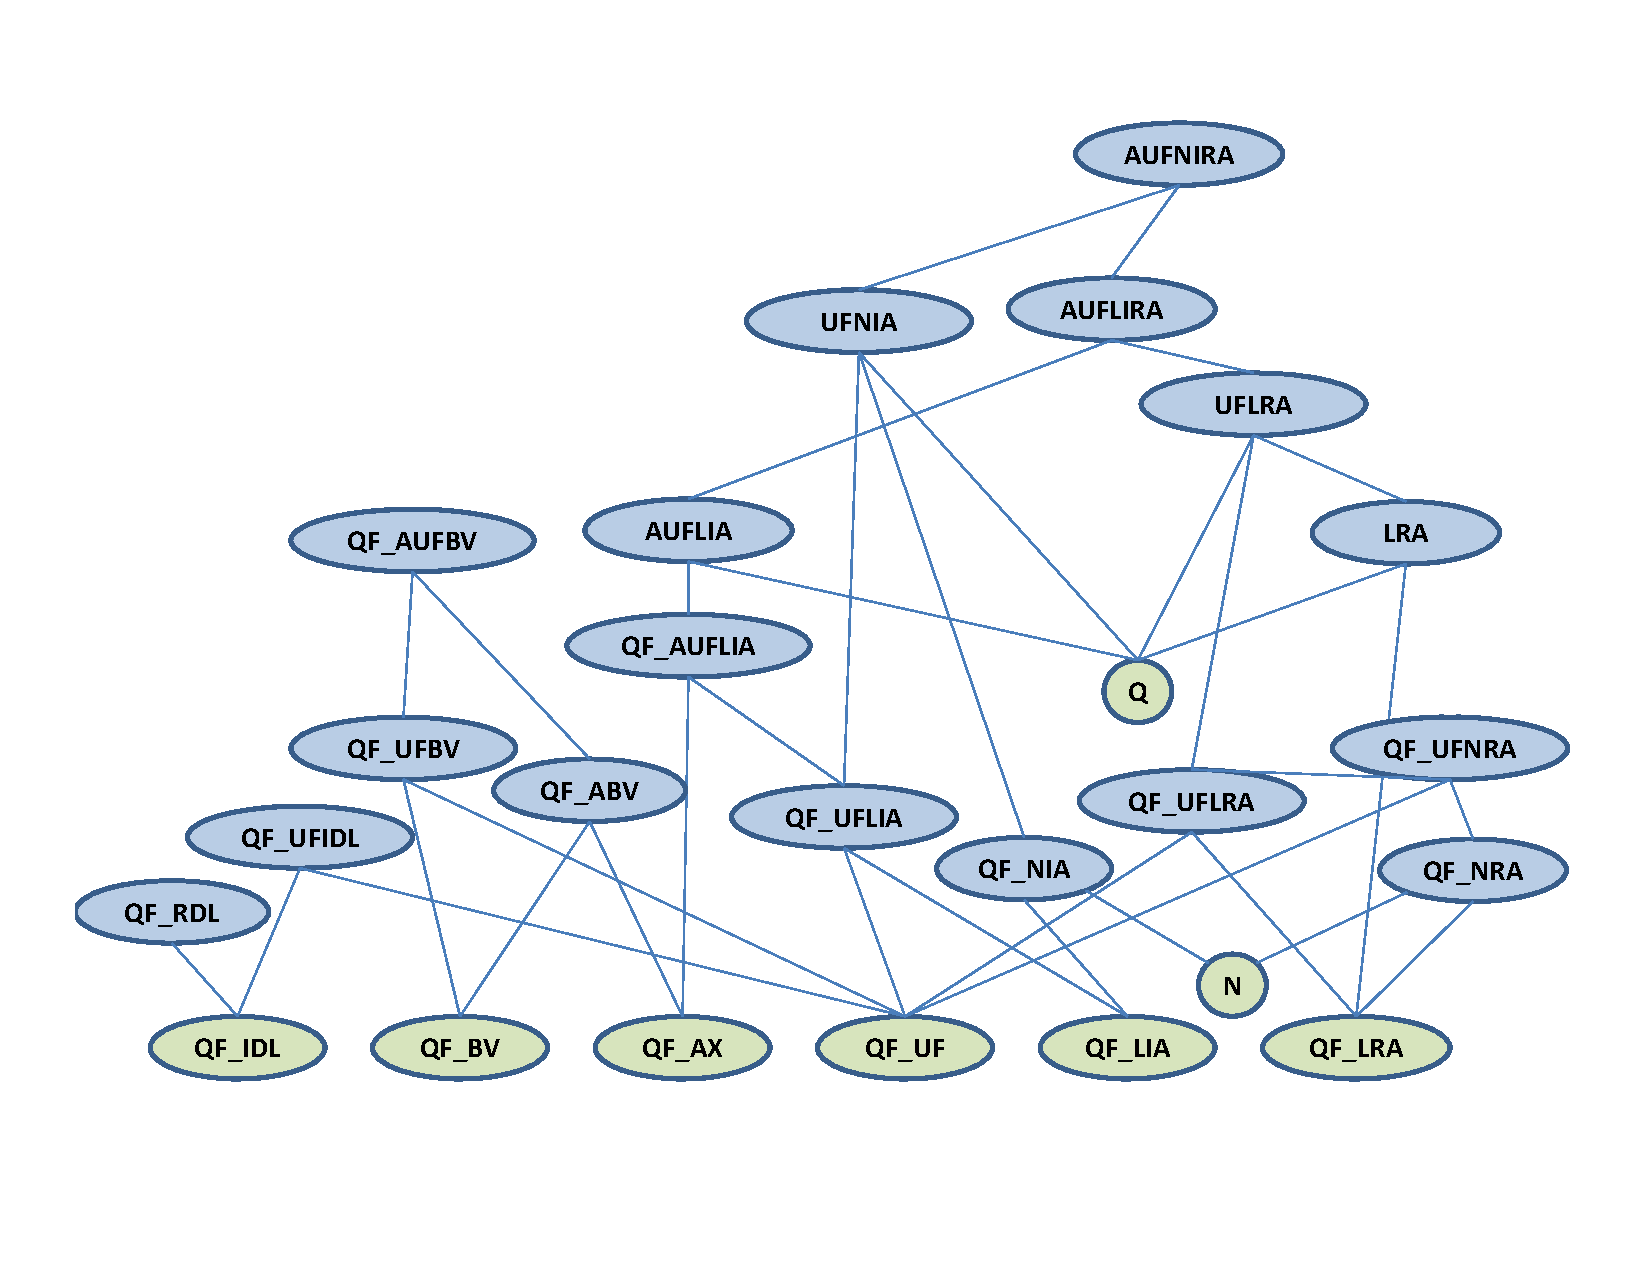
\includegraphics[width=\textwidth]{LogicLatticeN}
\caption{Lattice of SMT logics defined in SMT-LIB. The links represent a natural inclusion by characteristics, but {\it not} a sub-logic relationship. {\tt QF\_ABV} is defined, but is often subsumed in {\tt QF\_AUFBV}, and is not usually listed separately in other tables in this report. {\tt Q} is not a logic by itself but is a characteristic indicating that quantified expressions are permitted in the logic; similarly {\tt N} indicates non-linear arithmetic is allowed.}
\label{Fig:lattice}
\end{figure}

SMT-LIB defines a number of theories and logics. The logics are a combination of theories with additional functions or logic symbols or restrictions on the vocabulary of the theories. For example, the {\tt QF\_IDL} logic uses the underlying {\tt Ints} theory, but restricts terms to equalities and inequalities between constants and simple differences of variables.
The combination of the {\tt Ints} theory and the {\tt Reals} theory adds functions that convert between integers and reals (among other things). 
Note that the {\tt QF\_ABV} logic is defined, but is often subsumed in {\tt QF\_AUFBV} and has no benchmarks of its own;\footnote{By the time of the 2014 competition, the benchmarks were reorganized and recategorized, and more benchmarks were added. So now this logic is populated as well.} it is not usually listed separately in other tables in this report.

Leaving aside difference logics as special cases of integer and real logics, there are essentially these mostly orthogonal characteristics underlying the theories and logics:
\begin{itemize}[noitemsep,nolistsep] %% these modifiers are not supported in all document classes
\item IA: integers 
\item RA: reals
\item N: non-linear arithmetic
\item A or AX: arrays
\item UF: uninterpreted functions
\item QF\_: quantifier freeness
\item BV: bit-vectors
\end{itemize}
This list of characteristics partially corresponds to the set of SMT-LIB theories. The exceptions are quantification and non-linearity, both of which designate lifting restrictions on the kinds of terms allowed in the resulting logic. (Since they do not correspond exactly to underlying SMT theories, the term {\em characteristics} is used in this discussion.)

It is possible to define a logic with any powerset of these characteristics in an almost purely combinatorial sense. 
Barring non-linearity without arithmetic and the useless empty set, there are 111 combinations of characteristics (instead of the full 128). SMT-LIB has definitions and benchmarks for 20 of these logics (excluding QF\_RDL, QF\_IDL, and QF\_UFIDL) at the time of the evaluation, expanded to 34 in 2014. Fig.~\ref{Fig:lattice} shows what might be expected to be natural containment relationships among the logics defined at the time of this evaluation. 

However, what might be expected to be natural containment relationships are not actually sub-logic relationships. That more accurate relationship is shown in a diagram on the SMT-LIB website: \url{http://smtlib.cs.uiowa.edu/logics.shtml} (due to Cesare Tinelli). The principal cause of this lack of sub-logic relationship is that many of the logics supporting arrays support only specific sorts of arrays. For example, the basic QF\_AX logic allows arbitrary new sort symbols, including arrays over those free sorts. However, QF\_ABV (arrays and bit-vectors) does not allow new sort symbols and only allows arrays over bit-vector sorts.

The naming convention for logics is almost but not quite simply a combination of the letters indicated in the list above,
corresponding to the characteristics of the logic, with the letters listed in order by convention:
\begin{center}
{\tt [QF\_][A|AX][UF][BV][N|L][IA|RA|IRA]}.}
\end{center}

\noindent The non-uniformities are these:
\begin{itemize}[noitemsep,nolistsep]
\item quantification is indicated by {\em removing} a {\tt QF\_} prefix;
\item the absence of non-linearity ({\tt N}), i.e., linearity, is indicated by an {\tt L}, instead of by no designator; 
\item integer and real arithmetic are indicated by two letters ({\tt IA} and {\tt RA}) and their combination by {\tt IRA}; \item the {\tt A} used in the arithmetic designators could be ambiguous with the designator for arrays, except for position;
\item a logic with just arrays is named {\tt QF\_AX}, whereas in other combinations including arrays, just an {\tt A} instead of {\tt AX} is used.
\end{itemize}
For example, {\tt UFNIA} includes quantification (no {\tt QF\_} prefix), uninterpreted functions (UF), non-linearity (N), and integer arithmetic (IA), leaving out arrays, bit-vectors, and reals.

These names have roots in the history of development of SMT-LIB. Nevertheless as the set of logics grows -- 23 here and 34 by the 2014 competition -- the situation will increasingly confuse new users of SMT-LIB trying to understand the structure of logics; in addition new theories and accompanying logics are anticipated.
It would be useful to standardize the naming convention along the lines of current use, perhaps with slight adjustments (e.g., renaming {\tt QF\_AX} to {\tt QF\_A} and removing the excess {\tt A} from {\tt IA} and {\tt RA}), in order to define precisely the logic implied by any combination of designators. A policy regarding names would provide a process for defining names for new theories and logics. This would
also make it easier to accurately characterize new benchmarks and to summarize the logics supported by a given solver. This need has been raised to the SMT-LIB coordinators and some work has been started to address it.

%The absence of many combinations appears to be simply a matter of ad hoc lack of research or non-existence of benchmarks. For example,
%all five meaningful combinations of {\tt UF}, {\tt N} and {\tt RA} are present, but only four of the combinations of {\tt UF}, {\tt N} and {\tt IA}. Obviously there is no point to filling out all combinations, just for completeness. However,
%benchmarks could come in any form, and it would be useful to be able to categorize them precisely. The collection of benchmarks should be driven by technical interest and application need. With the exception of some of the needed conversions (e.g., between bitvectors and numbers), there seems little technical impediment to combining characteristics once the corresponding underlying theories and decision procedures are implemented. That leaves application need as a driver; this is discussed further in section \ref{Applications}. It is also conceivable that some logics should be deemphasized, either because solvers have progressed to such an extent that the logic no longer poses interesting technical questions or because applications have little need for the logic.

\subsection{Coverage of logics by solvers}
\label{Coverage}

\begin{figure}
\centering

\begin{tabular}{|l|p{.02in}p{.02in}p{.02in}p{.02in}p{.02in}p{.02in}p{.02in}p{.02in}p{.02in}p{.02in}p{.02in}p{.02in}p{.02in}p{.02in}p{.02in}p{.02in}p{.02in}p{.02in}p{.02in}p{.02in}p{.02in}p{.02in}|}
\hline
&  \rotatebox[origin=lB]{90}{AUFLIA} & \rotatebox[origin=lB]{90}{AUFLIRA} & \rotatebox[origin=lB]{90}{AUFNIRA} & \rotatebox[origin=lB]{90}{LRA} & \rotatebox[origin=lB]{90}{QF\_AUFBV} & \rotatebox[origin=lB]{90}{QF\_AUFLIA~} & \rotatebox[origin=lB]{90}{QF\_AX} & \rotatebox[origin=lB]{90}{QF\_BV} & \rotatebox[origin=lB]{90}{QF\_IDL} & \rotatebox[origin=lB]{90}{QF\_LIA} & \rotatebox[origin=lB]{90}{QF\_LRA} & \rotatebox[origin=lB]{90}{QF\_NIA} & \rotatebox[origin=lB]{90}{QF\_NRA} & \rotatebox[origin=lB]{90}{QF\_RDL} & \rotatebox[origin=lB]{90}{QF\_UF} & \rotatebox[origin=lB]{90}{QF\_UFBV} & \rotatebox[origin=lB]{90}{QF\_UFIDL} & \rotatebox[origin=lB]{90}{QF\_UFLIA} & \rotatebox[origin=lB]{90}{QF\_UFLRA} & \rotatebox[origin=lB]{90}{QF\_UFNRA} & \rotatebox[origin=lB]{90}{UFLRA} & \rotatebox[origin=lB]{90}{UFNIA} \\ \hline
4Simp-SMT-COMP-2012 (1)                  &   &   &   &   &   &   &   & X &   &   &   &   &   &   &   &   &   &   &   &   &   &     \\ \hline
Abziz... (5)                             &   &   &   &   &   &   &   & X &   &   &   &   &   &   &   &   &   &   &   &   &   &     \\ \hline
AProVE-NIA-SMT-COMP-2011 ... (2)         &   &   &   &   &   &   &   &   &   &   &   & X &   &   &   &   &   &   &   &   &   &     \\ \hline
Boolector-1.5.118-SMT-EVAL-2013 ... (3)  &   &   &   &   & \textbullet &   &   & \textbullet &   &   &   &   &   &   &   & \textbullet &   &   &   &   &   &     \\ \hline
CVC3-SMT-COMP-2012 ... (3)               & X & X & X & X & X & X & X & X & X & X & X & X & X & X & X & X & X & X & X & X & X & X    \\
CVC4-SMT-COMP-2010                       &   &   &   &   &   &   &   &   &   &   & X &   &   &   &   &   &   &   &   &   &   &     \\
CVC4-SMT-COMP-2011                       &   &   &   &   &   &   & X &   &   &   & X &   &   &   & X &   &   &   &   &   &   &     \\
CVC4-SMT-COMP-2012-Resubmission          & X & X &   & X & X & X & X & X & X & X & X &   &   & X & X & X & X & X & X &   & X &      \\
CVC4-SMT-EVAL-2013                       & \tb & \tb &   & \tb & \tb & \tb & \tb & \tb & \tb & \tb & \tb &   &   & \tb & \tb & \tb & \tb & \tb & \tb &   & \tb &      \\ \hline
MathSAT5-5.2.6-SMT-EVAL-2013             &   &   &   &   & \tb & \tb & \tb & \tb &   & \tb & \tb &   &   &   & \tb & \tb &   & \tb & \tb &   &   &      \\
MathSAT5-HeavyBV-SMT-COMP-2012           &   &   &   &   &   &   &   & X &   &   &   &   &   &   &   &   &   &   &   &   &   &     \\
MathSAT5-SMT-COMP-2010                   &   &   &   &   &   &   &   &   &   & X & X &   &   &   & X &   &   & X & X &   &   &     \\
MathSAT5-SMT-COMP-2011                   &   &   &   &   & X & X & X & X &   & X & X &   &   &   & X &   &   & X & X &   &   &     \\
MathSAT5-SMT-COMP-2012                   &   &   &   &   & X & X &   & X &   & X & X &   &   &   & X &   &   & X & X &   &   &     \\
test\_pmathsat-SMT-COMP-2010             &   &   &   &   &   &   &   &   &   & X & X &   &   &   & X &   &   & X & X &   &   &     \\ \hline
MiniSMT-0.5-SMT-EVAL-2013 ... (2)        &   &   &   &   &   &   &   &   &   &   &   & \tb & \tb &   &   &   &   &   &   &   &   &     \\ \hline
OpenSMT-SMT-COMP-2011 ... (2)            &   &   &   &   &   &   &   &   & X &   & X &   &   & X & X &   & X &   &   &   &   &     \\
OpenSMT-SMT-EVAL-2013                    &   &   &   &   &   &   &   &   &   &   &   &   &   &   & \tb &   &   &   &   &   &   &     \\ \hline
SMTInterpol-2.0r8402-SMT-EVAL-2013 ... (3)&   &   &   &   &   &   &   &   &   & \tb & \tb &   &   &   & \tb &   &   & \tb & \tb &   &   &     \\ \hline
SONOLAR-2013-05-15--SMT-EVAL-2013 ... (3)&   &   &   &   & \tb &   &   & \tb &   &   &   &   &   &   &   & \tb &   &   &   &   &   &     \\
SONOLAR-SMT-COMP-2010                    &   &   &   &   &   &   &   & X &   &   &   &   &   &   &   &   &   &   &   &   &   &     \\ \hline
STP2-SMT-COMP-2012 ... (3)               &   &   &   &   &   &   &   & X &   &   &   &   &   &   &   &   &   &   &   &   &   &     \\ \hline
TdW-SMT-COMP-2012                        &   &   &   &   & X &   &   &   &   &   &   &   &   &   &   &   &   &   &   &   &   &     \\ \hline
veriT-SMT-COMP-2010                      &   &   &   &   &   &   &   &   & X &   &   &   &   & X & X &   & X &   &   &   &   &     \\
veriT-SMT-COMP-2011                      &   &   &   &   &   &   &   &   & X &   &   &   &   & X & X &   & X &   &   &   &   &     \\
veriT-SMT-EVAL-2013                      & \tb & \tb &   &   &   & \tb &   &   & \tb & \tb & \tb &   & \tb & \tb & \tb &   & \tb & \tb & \tb & \tb & \tb &     \\ \hline
Z3-4.3.2.a054b099c1d6-x64-debian-6.0.6-SMT-EVAL-2013 (2)                               & \tb & \tb & \tb & \tb & \tb & \tb & \tb & \tb & \tb & \tb & \tb & \tb & \tb & \tb & \tb & \tb & \tb & \tb & \tb & \tb & \tb & \tb    \\ \hline
                                         &   &   &   &   &   &   &   &   &   &   &   &   &   &   &   &   &   &   &   &   &   &     \\ \hline
Total current (2013) solvers             & 3 & 3 & 1 & 2 & 5 & 4 & 3 & 5 & 3 & 5 & 5 & 2 & 3 & 3 & 6 & 5 & 3 & 5 & 5 & 2 & 3 & 1   \\ \hline
\end{tabular}

\caption{Support for each logic as stated by solver implementors. The dots instead of Xs identify the 2013 versions of solvers. The numbers in the bottom row are the number of 2013 solvers for each logic.}
\label{Fig:solversupport}
\end{figure}

Each solver supports some subset of the SMT logics and the corresponding theories and characteristics described in the previous section. The set of logics supported by solvers (as stated by the solver teams) is shown in Fig.~\ref{Fig:solversupport}. CVC and Z3 support all or nearly all logics, with CVC4 just missing full support for non-linear arithmetic (it does have partial support, with full support in the 2014 competition); veriT and MathSat support a significant number of logics.

The numbers in the bottom row of the figure state the number of current (2013) solvers that support a given logic. The characteristics most lacking are quantifiers and nonlinearity. Those with the most support are bitvectors, uninterpreted functions and arithmetic.

Note that the support indicated is that stated by the solver supplier at the time the solver was submitted to a competition. 
In some cases, a solver supports one logic but is not listed as supporting a subset of that logic. The general reason is that the subset, with restricted characteristics, allows for specific optimizations that are not implemented. The more general solver could act on problems of the
more restricted benchmarks but is not deemed competitive and thus was not formally entered into the competition for the restricted logic.


\subsection{Progress in solver performance}
\label{Progress}

We can obtain a measure of the overall year-by-year improvement in solver performance by applying each year's solvers to all the benchmarks (within each logic), observing the best performance on each benchmark. That is, the data shows a {\em virtual best performer}, obtained by an all-knowing oracle choosing, for each benchmark, the solver that performs best on that benchmark.

Fig.~\ref{Fig:CumulativeTimes} shows the fraction of benchmarks completed (y-axis) within a given time (in seconds, on the x-axis); thus points toward the upper left are better (more completed in less time). The results for all logics are shown together. 
The four curves are the data for the four years from 2010 to 2013. The lowest (marked with fine dots) curve is that for 2010. 
There is clearly significant progress made from 2010 to later years: the number of benchmarks completed within a given time is noticeably higher; we did not attempt to identify the source of this historical improvement. The curves for 2011 and 2012 (heavy dashes and short dashes, respectively) are clearly above 2010, but are not substantially different from each other. The solvers for 2013 (heavy solid line) are uniformly above those for previous years, but not by a large amount.  

By this data, the improvements in raw SMT solver performance on the current set of benchmark problems have slowed down, though they may have improved by other measures.

\begin{figure}
\centering
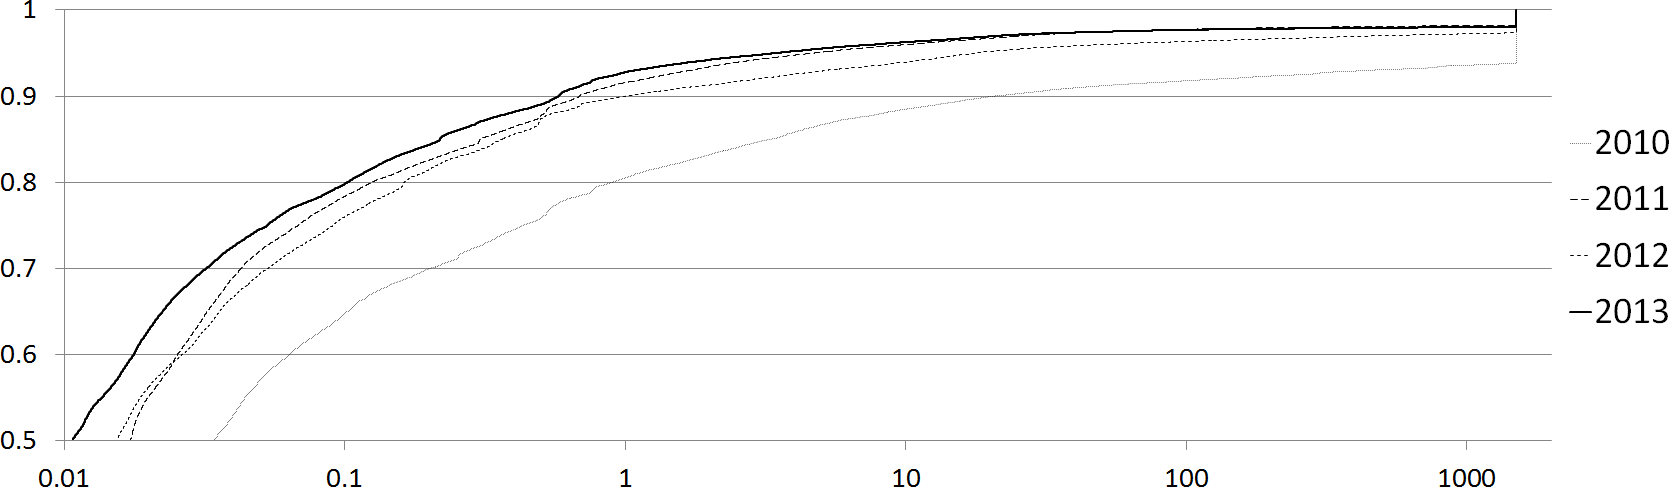
\includegraphics[width=.95\textwidth]{CumulativeTimes}
\caption{The fraction of benchmarks (y-axis) whose winning time is less than the given number of seconds (x-axis), by year.}
\label{Fig:CumulativeTimes}
\end{figure}

An alternate measure of solver progress is to count, for a given logic, what fraction of the benchmarks have a better time in a given year than in the previous year, by the best solver for each year. That data is shown in Fig.~\ref{Fig:bettertime}. Though most data points indicate that most benchmarks improved year to year, the progress is not uniform. The progress from 2010 to 2013 shows nearly all logics having improvement rates above 80\%, but there are definitely some laggards. There is not necessarily a monotonic improvement because the set of solvers is different from year to year; some well-performing solvers may choose not to participate every year.

\begin{figure}
\centering
%\begin{tabular}{|l|r|rrrr|}
%\hline
%Logic & \# benchmarks & 2010-2011 & 2011-2012 & 2012-2013 & 2010-2013\\ \hline
AUFLIA & 6402 & 90.83\% & 16.51\% & 85.16\% & 88.53\% \\
AUFLIRA & 19917 & 75.66\% & 64.97\% & 92.55\% & 95.37\% \\
AUFNIRA & 989 & 78.67\% & 61.48\% & 82.31\% & 86.65\% \\
LRA & 374 & 80.21\% & 94.65\% & 62.57\% & 91.44\% \\
QF\_AUFBV & 14335 & 95.33\% & 67.39\% & 50.77\% & 96.29\% \\
QF\_AUFLIA & 1140 & 87.11\% & 32.19\% & 91.67\% & 94.82\% \\
QF\_AX & 551 & 88.93\% & 29.76\% & 67.70\% & 84.39\% \\
QF\_BV & 31747 & 68.26\% & 66.87\% & 33.10\% & 66.66\% \\
QF\_IDL & 2170 & 83.46\% & 5.71\% & 85.44\% & 86.22\% \\
QF\_LIA & 5882 & 54.47\% & 58.98\% & 91.50\% & 84.99\% \\
QF\_LRA & 634 & 58.83\% & 40.06\% & 87.85\% & 87.22\% \\
QF\_NIA & 530 & 43.96\% & 10.57\% & 79.43\% & 45.85\% \\
QF\_NRA & 166 & 72.89\% & 19.28\% & 97.59\% & 95.78\% \\
QF\_RDL & 255 & 77.25\% & 4.31\% & 76.47\% & 58.43\% \\
QF\_UF & 6647 & 85.26\% & 6.27\% & 97.23\% & 93.62\% \\
QF\_UFBV & 31 & 100.00\% & 67.74\% & 32.26\% & 100.00\% \\
QF\_UFIDL & 430 & 94.88\% & 1.16\% & 97.21\% & 94.19\% \\
QF\_UFLIA & 564 & 91.13\% & 22.16\% & 92.02\% & 94.50\% \\
QF\_UFLRA & 900 & 51.44\% & 38.67\% & 94.33\% & 88.67\% \\
QF\_UFNRA & 26 & 100.00\% & 15.38\% & 100.00\% & 100.00\% \\
UFLRA & 5 & 100.00\% & 20.00\% & 20.00\% & 20.00\% \\
UFNIA & 1796 & 87.58\% & 11.41\% & 76.89\% & 80.85\% \\
\hline
TOTAL & 95491 & 76.87\% & 53.88\% & 65.32\% &  83.58\% \\
%\hline
%\end{tabular}
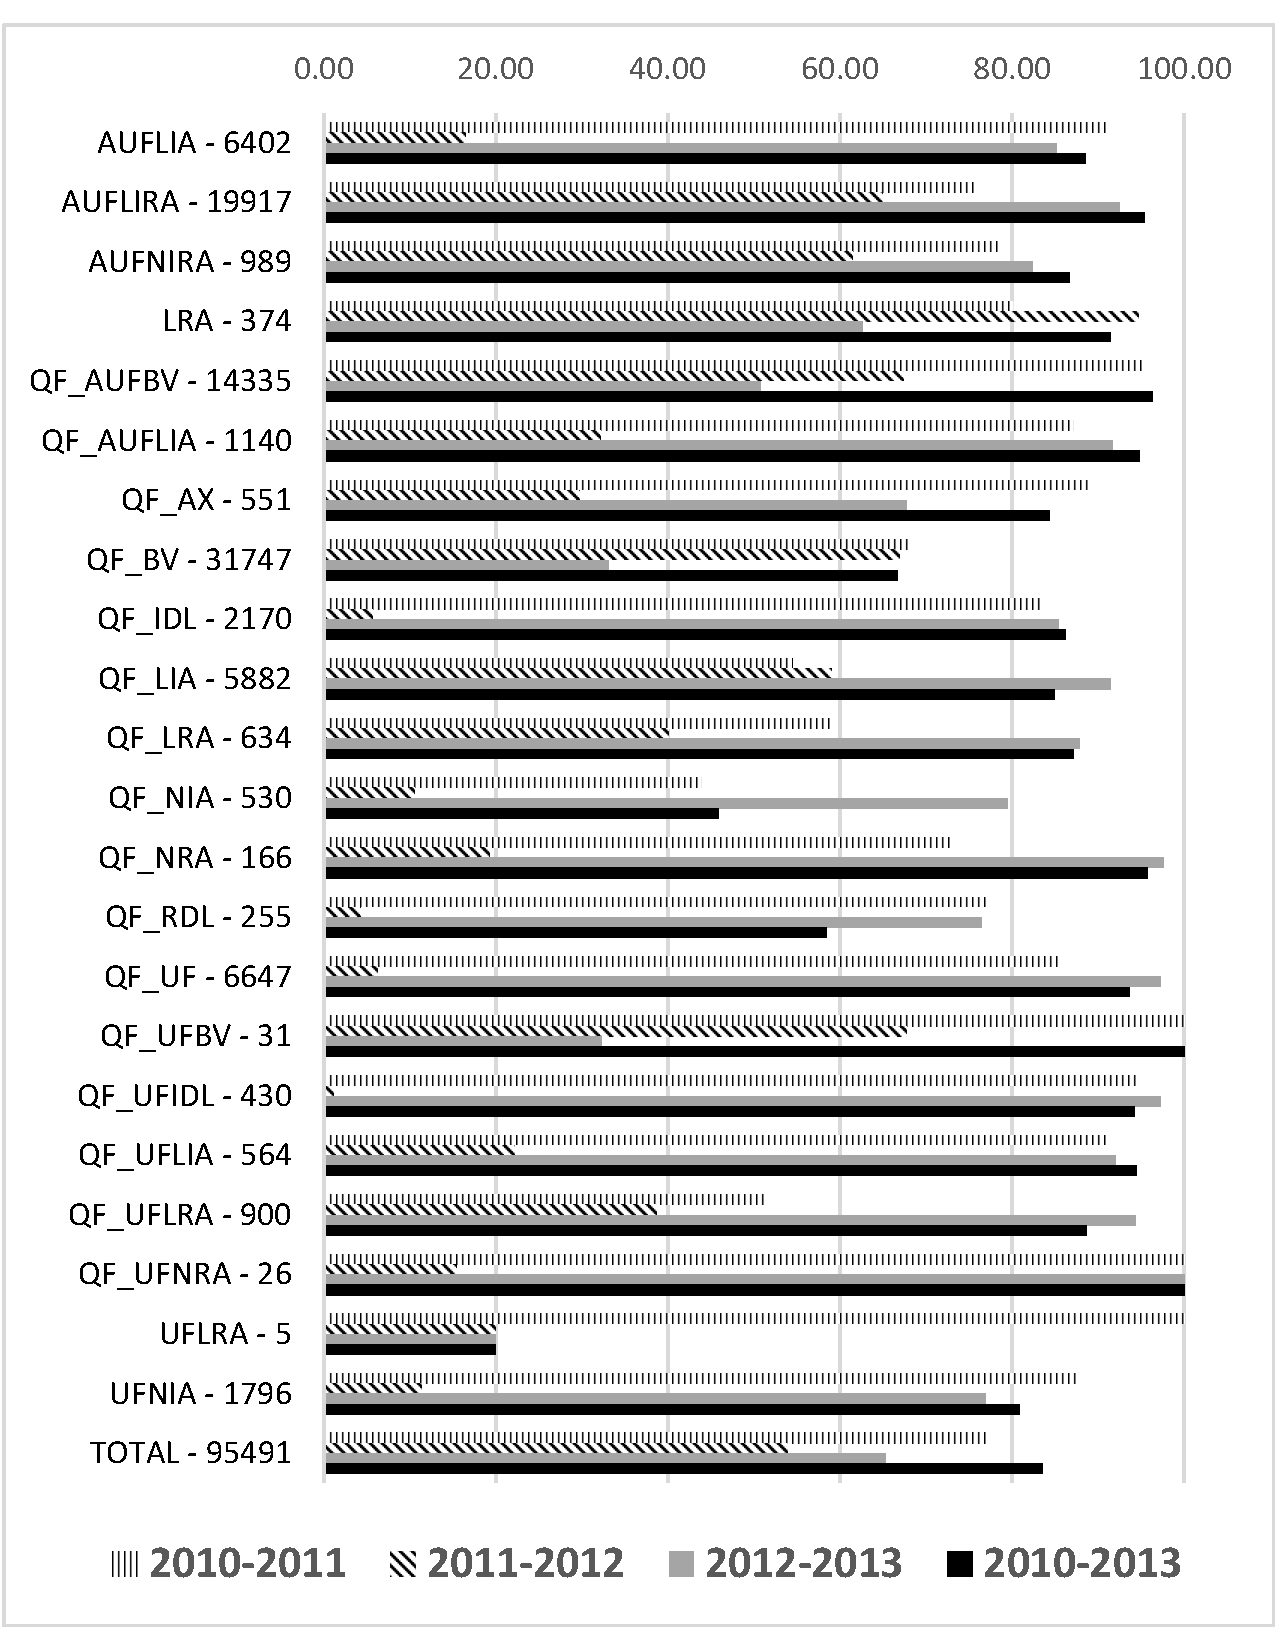
\includegraphics[width=\textwidth]{bettertime.pdf}
\caption{The fraction of benchmarks whose best time improved between the given years.}
\label{Fig:bettertime}
\end{figure}


\subsection{Repeatability of competitions}
\label{CompetitionRepeatability}

The SMT competition aims to be a repeatable measurement of relative performance of solvers. To that end the details of the competition, such as the rules and selection of benchmarks, are made public. In addition the solvers themselves are required to be made public after the competition.

However, there are aspects of the competition that are not deterministic. We measured two of those in this evaluation:
\begin{itemize}[noitemsep,nolistsep]
\item {\em The repeatability of the time a given solver takes on a given benchmark} (Section \ref{Accuracy}). This variation is a combination of two factors: any variation in execution and timing by the Star-Exec system itself, and any non-determinism in the execution of the solver.
\item {\em Variation caused by selection of benchmarks} (Section \ref{BenchmarkSelection}). \end{itemize}
 
 There is the additional risk that the set of benchmarks in SMT-LIB is not representative of any particular application area. 
We do not evaluate that risk here, but expect that this is quite likely the case.
As noted in our conclusions, we consider assessment of benchmarks as the most 
important aspect of future work. It would consist of a survey of the uses of SMT solvers, determination of the corresponding characteristics needed of solvers, an assessment of the degree to which current benchmarks are representative of the identified uses, and collection of additional benchmarks.

 
\subsubsection{Accuracy of performance measurements}
\label{Accuracy}

To measure the repeatability of a given solver on a given benchmark, we produced a random selection of benchmark-solver pairs (job-pairs), selecting only among job-pairs that did not timeout and had a running time of at least 0.1~seconds. The random selection produced 10\,165 job-pairs (out of the total 1\,663\,478 job-pairs). These job-pairs were run 8 times on 8 different days. Each such run took only a few hours. This resulted in 8 repetitions of each of the selected job-pairs. The data set is archived with the other evaluation data on the SMT-EVAL website. Star-Exec was lightly loaded on these days, so we did not measure any effect owing to interference with other uses of Star-Exec.

The 8 measured values for a job-pair were sorted and the first, median, and third quartile measured; these are as the average of sorted values 2 and 3, 4 and 5, and 6 and 7, respectively, and designated as Q1, Q2, and Q3. We noted the following points:
\begin{itemize}[noitemsep,nolistsep]
\item Of the measured job-pairs, about 78\% had an interquartile range (difference between Q3 and Q1) less than 10\% of the median value. That is, repeated measurements will fall within about 10\% of each other roughly 50\% of the time.\footnote{We did not measure skew: the degree to which Q3 and Q1 are unequally distant from the median.}
\item 3.5\% of job-pairs showed an interquartile range more than 50\% of the median value. 
\item Nine cases of the 10165 had a Q3 value more than double the median. These clearly showed multi-modal behavior among the eight data points for each benchmark-solver pair. Such behavior is likely the result of non-deterministic choices within the solver's search algorithms. 
\item We did not expand our study to determine whether the variation in performance was correlated to the choice of solver or to certain benchmarks. Also, we did not measure any effects owing to benchmark scrambling, which we now know can change solver behavior significantly.
\end{itemize}

An approximate conclusion from the above is that variation in timing itself plays a relatively small role in any variation in the competition. We expect the variation averages out over\ many benchmarks and is not correlated with particular solvers. It might have a larger effect on benchmarks with short running times (but we did not quantify this). The number of benchmarks per division used in previous competitions was on the order of 200, but did vary from division to division; the standard deviation of a mean calculated from a sample of 200 observations of an approximately normal distribution would be only about 0.05 of the interquartile range. 

Any variation due to non-determinism within a solver we consider part of that solver's design. Thus it is possible that in some competition a non-deterministic solver might do quite well, while in a repeat of the same competition that solver, making other internal random choices, might do poorly. 

\subsubsection{Accuracy of competitions}
\label{BenchmarkSelection}
The data we collected allows us to simulate various competition organizations. One such competition design would be, for each logic, to run all solvers for the given year on all benchmarks. The result of such an exercise is shown in Figs. \ref{Fig:virtual-competition-all} and \ref{Fig:virtual-competition-all2} for the set of 9 solvers for the year 2013. By summing all the CPU times for each benchmark-solver combination, we obtain that such a competition would use about 443 days of wall-clock time (using one computational node); for this computation we consider all timeout and memory exhaustion results to have taken the full timeout value (1500 sec) of time. It is possible that in some cases a solver may exhaust memory prior to the timeout.

In previous competitions, the winner was determined as the solver that correctly solved the most benchmarks within the timeout limit (solvers producing incorrect results are disqualified). Ties among solvers solving the same number of benchmarks are resolved in favor of the solver taking the least amount of time to produce its solutions. In the tables showing the results, for each logic, the results are reported in the order of a virtual winner.

\begin{figure}
\centering
\begin{tabular}{|p{.01in}rrl|}
\hline
 & \# unsolved & secs & solver \\
\hline
\multicolumn{4}{|l|}{AUFLIA 6402 benchmarks ,      71.53 days wall time} \\ 
 & 936 & 1404424.66 & Z3-4.3.2.a054b099c1d6-x64-debian-6.0.6-SMT-EVAL-2013 \\
 & 1278 & 1957553.10 & CVC4-SMT-EVAL-2013 \\
 & 1873 & 2818137.76 & veriT-SMT-EVAL-2013 \\
\hline
\multicolumn{4}{|l|}{AUFLIRA 19917 benchmarks ,      27.95 days wall time} \\ 
 & 254 & 389439.43 & Z3-4.3.2.a054b099c1d6-x64-debian-6.0.6-SMT-EVAL-2013 \\
 & 638 & 976484.46 & CVC4-SMT-EVAL-2013 \\
 & 680 & 1049109.48 & veriT-SMT-EVAL-2013 \\
\hline
\multicolumn{4}{|l|}{AUFNIRA 989 benchmarks ,       0.14 days wall time} \\ 
 & 8 & 12012.02 & Z3-4.3.2.a054b099c1d6-x64-debian-6.0.6-SMT-EVAL-2013 \\
\hline
\multicolumn{4}{|l|}{LRA 374 benchmarks ,       3.49 days wall time} \\ 
 & 68 & 105139.09 & Z3-4.3.2.a054b099c1d6-x64-debian-6.0.6-SMT-EVAL-2013 \\
 & 127 & 196132.91 & CVC4-SMT-EVAL-2013 \\
\hline
\multicolumn{4}{|l|}{QF\_AUFBV 14335 benchmarks ,      64.28 days wall time} \\ 
 & 520 & 805442.63 & Boolector-1.5.118-SMT-EVAL-2013 \\
 & 543 & 844767.74 & SONOLAR-2013-05-15-SMT-EVAL-2013 \\
 & 712 & 1106772.52 & Z3-4.3.2.a054b099c1d6-x64-debian-6.0.6-SMT-EVAL-2013 \\
 & 864 & 1332157.54 & MathSAT5-5.2.6-SMT-EVAL-2013 \\
 & 948 & 1465081.78 & CVC4-SMT-EVAL-2013 \\
\hline
\multicolumn{4}{|l|}{QF\_AUFLIA 1140 benchmarks ,       3.40 days wall time} \\ 
 & 16 & 24087.55 & veriT-SMT-EVAL-2013 \\
 & 23 & 34635.67 & Z3-4.3.2.a054b099c1d6-x64-debian-6.0.6-SMT-EVAL-2013 \\
 & 72 & 113550.39 & CVC4-SMT-EVAL-2013 \\
 & 81 & 121754.16 & MathSAT5-5.2.6-SMT-EVAL-2013 \\
\hline
\multicolumn{4}{|l|}{QF\_AX 551 benchmarks ,       1.39 days wall time} \\ 
 & 19 & 28520.99 & Z3-4.3.2.a054b099c1d6-x64-debian-6.0.6-SMT-EVAL-2013 \\
 & 23 & 34530.42 & MathSAT5-5.2.6-SMT-EVAL-2013 \\
 & 38 & 57088.31 & CVC4-SMT-EVAL-2013 \\
\hline
\multicolumn{4}{|l|}{QF\_BV 31747 benchmarks ,     127.04 days wall time} \\ 
 & 944 & 1491616.08 & Boolector-1.5.118-SMT-EVAL-2013 \\
 & 1102 & 1750286.98 & Z3-4.3.2.a054b099c1d6-x64-debian-6.0.6-SMT-EVAL-2013 \\
 & 1469 & 2471860.33 & MathSAT5-5.2.6-SMT-EVAL-2013 \\
 & 1590 & 2498512.90 & SONOLAR-2013-05-15-SMT-EVAL-2013 \\
 & 1699 & 2763975.38 & CVC4-SMT-EVAL-2013 \\
\hline
\multicolumn{4}{|l|}{QF\_IDL 2170 benchmarks ,      27.81 days wall time} \\ 
 & 231 & 407530.76 & Z3-4.3.2.a054b099c1d6-x64-debian-6.0.6-SMT-EVAL-2013 \\
 & 360 & 689225.35 & CVC4-SMT-EVAL-2013 \\
 & 751 & 1305966.10 & veriT-SMT-EVAL-2013 \\
\hline
\multicolumn{4}{|l|}{QF\_LIA 5882 benchmarks ,      86.65 days wall time} \\ 
 & 172 & 340070.98 & MathSAT5-5.2.6-SMT-EVAL-2013 \\
 & 316 & 614640.90 & SMTInterpol-2.0r8402-SMT-EVAL-2013 \\
 & 366 & 646587.14 & Z3-4.3.2.a054b099c1d6-x64-debian-6.0.6-SMT-EVAL-2013 \\
 & 761 & 1482588.14 & CVC4-SMT-EVAL-2013 \\
 & 2910 & 4403063.03 & veriT-SMT-EVAL-2013 \\
\hline
\multicolumn{4}{|l|}{QF\_LRA 634 benchmarks ,       2.96 days wall time} \\ 
 & 7 & 15398.96 & CVC4-SMT-EVAL-2013 \\
 & 19 & 33604.65 & Z3-4.3.2.a054b099c1d6-x64-debian-6.0.6-SMT-EVAL-2013 \\
 & 23 & 43613.79 & MathSAT5-5.2.6-SMT-EVAL-2013 \\
 & 36 & 80377.24 & veriT-SMT-EVAL-2013 \\
 & 37 & 82658.86 & SMTInterpol-2.0r8402-SMT-EVAL-2013 \\
\hline
\multicolumn{4}{|l|}{QF\_NIA 530 benchmarks ,       3.26 days wall time} \\ 
 & 17 & 28080.56 & MiniSMT-0.5-SMT-EVAL-2013 \\
 & 160 & 253992.63 & Z3-4.3.2.a054b099c1d6-x64-debian-6.0.6-SMT-EVAL-2013 \\
\hline

\end{tabular}
\caption{(Part 1) Results of a virtual competition using the 2013 solvers on all benchmarks.}
\label{Fig:virtual-competition-all}
\end{figure}

\begin{figure}
\centering
\begin{tabular}{|p{.01in}rrl|}
\hline
 & \# unsolved & secs & solver \\
\hline
\multicolumn{4}{|l|}{QF\_NRA 166 benchmarks ,       1.64 days wall time} \\ 
 & 0 & 1.64 & veriT-SMT-EVAL-2013 \\
 & 12 & 22751.00 & MiniSMT-0.5-SMT-EVAL-2013 \\
 & 79 & 118521.63 & Z3-4.3.2.a054b099c1d6-x64-debian-6.0.6-SMT-EVAL-2013 \\
\hline
\multicolumn{4}{|l|}{QF\_RDL 255 benchmarks ,       2.57 days wall time} \\ 
 & 39 & 64875.77 & CVC4-SMT-EVAL-2013 \\
 & 39 & 65459.76 & Z3-4.3.2.a054b099c1d6-x64-debian-6.0.6-SMT-EVAL-2013 \\
 & 51 & 91419.17 & veriT-SMT-EVAL-2013 \\
\hline
\multicolumn{4}{|l|}{QF\_UF 6647 benchmarks ,      12.56 days wall time} \\ 
 & 30 & 46692.19 & veriT-SMT-EVAL-2013 \\
 & 62 & 106340.93 & CVC4-SMT-EVAL-2013 \\
 & 105 & 172032.14 & MathSAT5-5.2.6-SMT-EVAL-2013 \\
 & 111 & 171953.63 & Z3-4.3.2.a054b099c1d6-x64-debian-6.0.6-SMT-EVAL-2013 \\
 & 136 & 237594.15 & SMTInterpol-2.0r8402-SMT-EVAL-2013 \\
 & 183 & 350598.34 & OpenSMT-SMT-EVAL-2013 \\
\hline
\multicolumn{4}{|l|}{QF\_UFBV 31 benchmarks ,       0.79 days wall time} \\ 
 & 0 & 0.32 & Boolector-1.5.118-SMT-EVAL-2013 \\
 & 0 & 0.33 & SONOLAR-2013-05-15-SMT-EVAL-2013 \\
 & 7 & 15962.85 & Z3-4.3.2.a054b099c1d6-x64-debian-6.0.6-SMT-EVAL-2013 \\
 & 12 & 23942.91 & MathSAT5-5.2.6-SMT-EVAL-2013 \\
 & 18 & 28678.86 & CVC4-SMT-EVAL-2013 \\
\hline
\multicolumn{4}{|l|}{QF\_UFIDL 430 benchmarks ,       1.90 days wall time} \\ 
 & 7 & 11947.79 & Z3-4.3.2.a054b099c1d6-x64-debian-6.0.6-SMT-EVAL-2013 \\
 & 32 & 71695.10 & CVC4-SMT-EVAL-2013 \\
 & 46 & 80562.09 & veriT-SMT-EVAL-2013 \\
\hline
\multicolumn{4}{|l|}{QF\_UFLIA 564 benchmarks ,       2.03 days wall time} \\ 
 & 0 & 100.67 & Z3-4.3.2.a054b099c1d6-x64-debian-6.0.6-SMT-EVAL-2013 \\
 & 0 & 355.30 & MathSAT5-5.2.6-SMT-EVAL-2013 \\
 & 0 & 1090.59 & CVC4-SMT-EVAL-2013 \\
 & 0 & 1469.57 & SMTInterpol-2.0r8402-SMT-EVAL-2013 \\
 & 68 & 172440.25 & veriT-SMT-EVAL-2013 \\
\hline
\multicolumn{4}{|l|}{QF\_UFLRA 900 benchmarks ,       0.02 days wall time} \\ 
 & 0 & 40.09 & MathSAT5-5.2.6-SMT-EVAL-2013 \\
 & 0 & 40.86 & Z3-4.3.2.a054b099c1d6-x64-debian-6.0.6-SMT-EVAL-2013 \\
 & 0 & 57.85 & CVC4-SMT-EVAL-2013 \\
 & 0 & 162.95 & veriT-SMT-EVAL-2013 \\
 & 0 & 1246.65 & SMTInterpol-2.0r8402-SMT-EVAL-2013 \\
\hline
\multicolumn{4}{|l|}{QF\_UFNRA 26 benchmarks ,       0.12 days wall time} \\ 
 & 0 & 0.25 & veriT-SMT-EVAL-2013 \\
 & 4 & 10565.17 & Z3-4.3.2.a054b099c1d6-x64-debian-6.0.6-SMT-EVAL-2013 \\
\hline
\multicolumn{4}{|l|}{UFLRA 5 benchmarks ,       0.11 days wall time} \\ 
 & 0 & 39.29 & CVC4-SMT-EVAL-2013 \\
 & 2 & 3103.69 & Z3-4.3.2.a054b099c1d6-x64-debian-6.0.6-SMT-EVAL-2013 \\
 & 4 & 6300.71 & veriT-SMT-EVAL-2013 \\
\hline
\multicolumn{4}{|l|}{UFNIA 1796 benchmarks ,       1.55 days wall time} \\ 
 & 68 & 133752.97 & Z3-4.3.2.a054b099c1d6-x64-debian-6.0.6-SMT-EVAL-2013 \\
\hline
\end{tabular}
\caption{(Part 2) Results of a virtual competition using the 2013 solvers on all benchmarks.}
\label{Fig:virtual-competition-all2}
\end{figure}

%\begin{figure}
%\centering
%\begin{tabular}{|p{.1in}rrl|}
%\hline
% & \# unsolved & secs & solver \\
\hline
\multicolumn{4}{|l|}{QF\_UFLIA 564 benchmarks ,       2.03 days cpu time} \\ 
 & 0 & 100.67 & Z3-4.3.2.a054b099c1d6-x64-debian-6.0.6-SMT-EVAL-2013 \\
 & 0 & 355.30 & MathSAT5-5.2.6-SMT-EVAL-2013 \\
 & 0 & 1090.59 & CVC4-SMT-EVAL-2013 \\
 & 0 & 1469.57 & SMTInterpol-2.0r8402-SMT-EVAL-2013 \\
 & 68 & 172440.25 & veriT-SMT-EVAL-2013 \\
\hline
\multicolumn{4}{|l|}{QF\_UFLRA 900 benchmarks ,       0.02 days cpu time} \\ 
 & 0 & 40.09 & MathSAT5-5.2.6-SMT-EVAL-2013 \\
 & 0 & 40.86 & Z3-4.3.2.a054b099c1d6-x64-debian-6.0.6-SMT-EVAL-2013 \\
 & 0 & 57.85 & CVC4-SMT-EVAL-2013 \\
 & 0 & 162.95 & veriT-SMT-EVAL-2013 \\
 & 0 & 1246.65 & SMTInterpol-2.0r8402-SMT-EVAL-2013 \\
\hline
\multicolumn{4}{|l|}{QF\_UFNRA 26 benchmarks ,       0.12 days cpu time} \\ 
 & 0 & 0.25 & veriT-SMT-EVAL-2013 \\
 & 4 & 10565.17 & Z3-4.3.2.a054b099c1d6-x64-debian-6.0.6-SMT-EVAL-2013 \\
\hline
\multicolumn{4}{|l|}{UFLRA 5 benchmarks ,       0.11 days cpu time} \\ 
 & 0 & 39.29 & CVC4-SMT-EVAL-2013 \\
 & 2 & 3103.69 & Z3-4.3.2.a054b099c1d6-x64-debian-6.0.6-SMT-EVAL-2013 \\
 & 4 & 6300.71 & veriT-SMT-EVAL-2013 \\
\hline
\multicolumn{4}{|l|}{UFNIA 1796 benchmarks ,       1.55 days cpu time} \\ 
 & 68 & 133752.97 & Z3-4.3.2.a054b099c1d6-x64-debian-6.0.6-SMT-EVAL-2013 \\
\hline

%\end{tabular}
%\caption{(Part 3) Results of a virtual competition using the 2013 solvers on all benchmarks.}
%\label{Fig:virtual-competition-all3}
%\end{figure}

However, past competitions have not used all benchmarks, but rather a random subset of a selection of the benchmarks. It is worth asking how susceptible the competition results are to the particular subset of benchmarks used for the competition. Typically, the choice was not completely random; rather, the distribution was (a) constrained to have roughly equal representation of various categories of difficulty and (b) curated to avoid over-representation of benchmark families that contained many similar benchmarks. For our evaluation here, we determined the results of a virtual competition by simply randomly selecting different equal-sized subsets (ignoring difficulty measures), determining the competition results for each, and observing whether the competition results vary significantly depending on the subset.  Fig.~\ref{Fig:virtual-competition-some} shows the result of an experiment in which a virtual competition was executed on 1000 random subsets; we tallied the fraction of times that the winner was different than the winner in the full virtual competition (Figs. \ref{Fig:virtual-competition-all} - \ref{Fig:virtual-competition-all2}) and the fraction of times that the complete order of the finishers was different. (We limited our consideration to those logics with at least 100 benchmarks and with more than one solver.)

Note that we did not curate the benchmarks to address the issue of over-represent-ation of some benchmark families (the authors of this report are not knowledgeable about which families are at issue); we simply used all of the benchmarks.  Thus the study should not be seen as a competition that ranks solvers, but as one that investigates various competition organizations.

The results are quite instructive. In many logics, the competition winners change in only a small fraction of trials.
However, in several logics, the fraction of trials in which the winner changes is quite significant, in some cases over~60\%. Inspection of the data reveals two contributing causes.
\begin{itemize}
\item First, some logics have a relatively large number of benchmarks that are unsolved by some solver within the timeout limit.  The fraction of benchmarks that are not solved is shown in the final column of Fig.~\ref{Fig:virtual-competition-some} (this is the average fraction over all the solvers for that logic). Random selection of benchmarks can readily change the subset of unsolved benchmarks included in the virtual competition or change the balance of benchmarks solved by one solver vs. another. Since ``winning'' the virtual competition is determined primarily by the number of benchmarks solved, rather than the time, any change in the relative number of solved benchmarks may change the order of winners. 

For example, the logic QF\_AUFBV has 14335 benchmarks. Of those, 520 are unsolved by Boolector and 543 are unsolved by SONOLAR (the winner and runner up of the virtual competition). Of these only 346 are unsolved by both, leaving 174 unsolved only by Boolector and 197 unsolved only by SONOLAR. Choosing 1433 benchmarks at random, over 1000 trials, yields more benchmarks unsolvable by Boolector about 31\% of the time, more unsolved by SONOLAR about 62\% of the time, and the same about 7\% of the time. Thus, the random selection of the competition benchmark set would allow SONOLAR to best Boolector about 1/3 of the time, despite Boolector being better on the overall benchmark population for this logic.

\item Second, even when unsolved benchmarks are not a contributing factor, some pairs of solvers have total times that are close. Variations in time caused by slightly different choices of benchmarks might cause changes in winning order. The experiment described next explores this phenomenon further.

\end{itemize}

A second virtual competition can be run using only benchmarks that all competitors solved within the timeout period. This would not make a useful real competition because the result could be easily gamed: a solver could win by thoroughly optimizing performance on a few benchmarks and purposely not solving the remainder. However, in this evaluation, no solver has had the chance to do that; performing this evaluation allows comparing running times alone, without the additional factor of unsolved benchmarks.

Figs.~\ref{Fig:virtual-competition-solved} and \ref{Fig:virtual-competition-solved2} show the result of such a competition, for the nine 2013 solvers; it uses all benchmarks that all the solvers registered for a given logic solve. In addition we performed the same experiment of 1000 virtual competitions each using 10\% of these benchmarks.  Fig.~\ref{Fig:virtual-competition-solved-some} shows the variation in winning order across these trials. The variation is even more than that shown in Fig.~\ref{Fig:virtual-competition-some}. To obtain some insight into this variation, we tabulate, in columns~2 and~3 of Fig.~\ref{Fig:virtual-competition-solved}ff, the mean and standard deviation\footnote{This is the population standard devation. To obtain the sample standard deviation scale these values by $\sqrt{0.999}$ } of the total solution time for each of the solvers in each logic. The standard deviations are substantial compared to the differences in mean times between competing solvers; even though the distributions of solving times are not necessarily Gaussian, the data indicate a substantial probability that the order would change based solely on the random choice of benchmark subset.

\begin{figure}
\centering
\begin{tabular}{|lrr|rr|r|}
\hline
Logic & Benchmarks used & \#~Trials & \cellbr{Winner\\changed} & \cellbr{Order\\changed} & \cellbr{Avg.~not\\solved} \\ \hline
AUFLIA & 640\,/\,6402 & 1000 &   0.0\% &   0.0\%  &  0.213 \\
AUFLIRA & 1991\,/\,19917 & 1000 &   0.0\% &  30.9\%  &  0.026 \\
LRA & 37\,/\,374 & 1000 &   4.6\% &   4.6\%  &  0.261 \\
QF\_AUFBV & 1433\,/\,14335 & 1000 &  33.6\% &  46.7\%  &  0.050 \\
QF\_AUFLIA & 114\,/\,1140 & 1000 &  24.1\% &  58.4\%  &  0.042 \\
QF\_AX & 55\,/\,551 & 1000 &  33.6\% &  48.0\%  &  0.048 \\
QF\_BV & 3174\,/\,31747 & 1000 &   2.4\% &  26.7\%  &  0.043 \\
QF\_IDL & 217\,/\,2170 & 1000 &   0.0\% &   0.0\%  &  0.206 \\
QF\_LIA & 588\,/\,5882 & 1000 &   0.3\% &  24.4\%  &  0.154 \\
QF\_LRA & 63\,/\,634 & 1000 &  13.4\% &  67.7\%  &  0.038 \\
QF\_NIA & 53\,/\,530 & 1000 &   0.0\% &   0.0\%  &  0.167 \\
QF\_NRA & 16\,/\,166 & 1000 &   0.0\% &   0.0\%  &  0.183 \\
QF\_RDL & 25\,/\,255 & 1000 &  67.8\% &  70.8\%  &  0.169 \\
QF\_UF & 664\,/\,6647 & 1000 &   8.0\% &  71.1\%  &  0.016 \\
QF\_UFIDL & 43\,/\,430 & 1000 &   0.0\% &  18.2\%  &  0.066 \\
QF\_UFLIA & 56\,/\,564 & 1000 &   1.5\% &  24.6\%  &  0.024 \\
QF\_UFLRA & 90\,/\,900 & 1000 &  63.2\% &  68.8\%  &  0.000 \\
\hline

\end{tabular}
\caption{Results of virtual competitions using the 2013 solvers on random subsets of 10\% of the benchmarks.}
\label{Fig:virtual-competition-some}
\end{figure}

\begin{figure}
\centering
\begin{tabular}{|p{.01in}rrrl|}
\hline
 & total secs & \cellbr{mean\\for 10\%} & \cellbr{s.dev\\for 10\%} & solver \\
\hline
\multicolumn{5}{|l|}{AUFLIA 4174 benchmarks ,       0.22 days wall time} \\ 
 & 134.84 &     13.57 &      1.47 & Z3-4.3.2.a054b099c1d6-x64-debian-... \\
 & 8572.19 &    881.87 &    725.38 & veriT-SMT-EVAL-2013 \\
 & 10524.23 &   1017.33 &    644.67 & CVC4-SMT-EVAL-2013 \\
\hline
\multicolumn{5}{|l|}{AUFLIRA 18699 benchmarks ,       0.35 days wall time} \\ 
 & 239.75 &     23.99 &      1.14 & Z3-4.3.2.a054b099c1d6-x64-debian-... \\
 & 1190.59 &    113.12 &    245.28 & CVC4-SMT-EVAL-2013 \\
 & 29062.40 &   2906.81 &   1592.05 & veriT-SMT-EVAL-2013 \\
\hline
\multicolumn{5}{|l|}{LRA 209 benchmarks ,       0.10 days wall time} \\ 
 & 3104.20 &    308.70 &    505.21 & Z3-4.3.2.a054b099c1d6-x64-debian-... \\
 & 5619.18 &    531.80 &    581.02 & CVC4-SMT-EVAL-2013 \\
\hline
\multicolumn{5}{|l|}{QF\_AUFBV 12796 benchmarks ,       1.09 days wall time} \\ 
 & 9132.25 &    927.34 &    667.35 & Boolector-1.5.118-SMT-EVAL-2013 \\
 & 15551.14 &   1571.56 &    789.27 & MathSAT5-5.2.6-SMT-EVAL-2013 \\
 & 18228.79 &   1858.63 &    915.22 & Z3-4.3.2.a054b099c1d6-x64-debian-... \\
 & 19760.57 &   1997.13 &   1010.26 & SONOLAR-2013-05-15-SMT-EVAL-2013 \\
 & 31608.01 &   3146.44 &   1223.43 & CVC4-SMT-EVAL-2013 \\
\hline
\multicolumn{5}{|l|}{QF\_AUFLIA 1015 benchmarks ,       0.07 days wall time} \\ 
 & 33.34 &      3.32 &      1.52 & veriT-SMT-EVAL-2013 \\
 & 93.14 &      9.25 &     11.90 & Z3-4.3.2.a054b099c1d6-x64-debian-... \\
 & 206.75 &     20.42 &     11.43 & MathSAT5-5.2.6-SMT-EVAL-2013 \\
 & 5529.68 &    542.85 &    517.03 & CVC4-SMT-EVAL-2013 \\
\hline
\multicolumn{5}{|l|}{QF\_AX 491 benchmarks ,       0.00 days wall time} \\ 
 & 19.87 &      1.97 &      1.48 & Z3-4.3.2.a054b099c1d6-x64-debian-... \\
 & 27.64 &      2.76 &      1.28 & MathSAT5-5.2.6-SMT-EVAL-2013 \\
 & 86.80 &      8.57 &      8.89 & CVC4-SMT-EVAL-2013 \\
\hline
\multicolumn{5}{|l|}{QF\_BV 28981 benchmarks ,       5.95 days wall time} \\ 
 & 24741.62 &   2466.39 &    574.41 & Boolector-1.5.118-SMT-EVAL-2013 \\
 & 33090.65 &   3315.48 &    924.08 & Z3-4.3.2.a054b099c1d6-x64-debian-... \\
 & 58252.81 &   5780.94 &   1699.68 & SONOLAR-2013-05-15-SMT-EVAL-2013 \\
 & 180688.61 &  18097.26 &   2555.59 & CVC4-SMT-EVAL-2013 \\
 & 217464.30 &  21676.36 &   2996.98 & MathSAT5-5.2.6-SMT-EVAL-2013 \\
\hline
\multicolumn{5}{|l|}{QF\_IDL 1407 benchmarks ,       2.45 days wall time} \\ 
 & 10837.79 &   1075.06 &    400.21 & Z3-4.3.2.a054b099c1d6-x64-debian-... \\
 & 28005.20 &   2794.68 &    804.94 & CVC4-SMT-EVAL-2013 \\
 & 173260.34 &  17004.68 &   2911.07 & veriT-SMT-EVAL-2013 \\
\hline
\multicolumn{5}{|l|}{QF\_LIA 2085 benchmarks ,       1.18 days wall time} \\ 
 & 5108.99 &    517.56 &    288.02 & MathSAT5-5.2.6-SMT-EVAL-2013 \\
 & 9989.45 &   1026.38 &    847.97 & Z3-4.3.2.a054b099c1d6-x64-debian-... \\
 & 23068.05 &   2333.97 &   1019.42 & CVC4-SMT-EVAL-2013 \\
 & 30542.46 &   3107.09 &   1214.87 & veriT-SMT-EVAL-2013 \\
 & 33029.34 &   3264.05 &   1243.38 & SMTInterpol-2.0r8402-SMT-EVAL-2013 \\
\hline
\multicolumn{5}{|l|}{QF\_LRA 583 benchmarks ,       0.60 days wall time} \\ 
 & 1410.69 &    138.20 &     57.97 & Z3-4.3.2.a054b099c1d6-x64-debian-... \\
 & 2108.31 &    206.48 &     99.11 & CVC4-SMT-EVAL-2013 \\
 & 3892.58 &    394.05 &    395.39 & MathSAT5-5.2.6-SMT-EVAL-2013 \\
 & 21918.95 &   2141.70 &   1153.96 & SMTInterpol-2.0r8402-SMT-EVAL-2013 \\
 & 22838.44 &   2236.65 &   1019.30 & veriT-SMT-EVAL-2013 \\
\hline
\multicolumn{5}{|l|}{QF\_NIA 357 benchmarks ,       0.19 days wall time} \\ 
 & 2474.66 &    233.56 &    284.13 & MiniSMT-0.5-SMT-EVAL-2013 \\
 & 13683.23 &   1333.87 &    938.66 & Z3-4.3.2.a054b099c1d6-x64-debian-... \\\hline

\end{tabular}
\caption{(Part 1) A virtual competition run only on benchmarks that all solvers solve.}
\label{Fig:virtual-competition-solved}
\end{figure}

\begin{figure}
\centering
\begin{tabular}{|p{.01in}rrrl|}
\hline
 & total secs & \cellbr{mean\\for 10\%} & \cellbr{s.dev\\for 10\%} & solver \\

\hline
\multicolumn{5}{|l|}{QF\_NRA 87 benchmarks ,       0.01 days wall time} \\ 
 & 0.84 & &  & veriT-SMT-EVAL-2013 \\
 & 21.63 & &  & Z3-4.3.2.a054b099c1d6-x64-debian-... \\
 & 548.45 & &  & MiniSMT-0.5-SMT-EVAL-2013 \\
\hline
\multicolumn{5}{|l|}{QF\_RDL 203 benchmarks ,       0.24 days wall time} \\ 
 & 2759.19 &    255.65 &    229.84 & Z3-4.3.2.a054b099c1d6-x64-debian-... \\
 & 3296.74 &    319.74 &    161.95 & CVC4-SMT-EVAL-2013 \\
 & 14350.83 &   1404.44 &    870.90 & veriT-SMT-EVAL-2013 \\
\hline
\multicolumn{5}{|l|}{QF\_UF 6332 benchmarks ,       1.27 days wall time} \\ 
 & 878.33 &     87.54 &     10.37 & veriT-SMT-EVAL-2013 \\
 & 2740.19 &    266.55 &    285.91 & Z3-4.3.2.a054b099c1d6-x64-debian-... \\
 & 5374.81 &    525.67 &    428.07 & MathSAT5-5.2.6-SMT-EVAL-2013 \\
 & 5420.78 &    551.93 &    483.45 & CVC4-SMT-EVAL-2013 \\
 & 20575.64 &   2039.15 &    507.66 & SMTInterpol-2.0r8402-SMT-EVAL-2013 \\
 & 74537.24 &   7344.50 &   1841.05 & OpenSMT-SMT-EVAL-2013 \\
\hline
\multicolumn{5}{|l|}{QF\_UFBV 12 benchmarks ,       0.03 days wall time} \\ 
 & 0.11 & &  & Boolector-1.5.118-SMT-EVAL-2013 \\
 & 0.13 & &  & SONOLAR-2013-05-15-SMT-EVAL-2013 \\
 & 312.28 & &  & Z3-4.3.2.a054b099c1d6-x64-debian-... \\
 & 786.01 & &  & MathSAT5-5.2.6-SMT-EVAL-2013 \\
 & 1625.99 & &  & CVC4-SMT-EVAL-2013 \\
\hline
\multicolumn{5}{|l|}{QF\_UFIDL 382 benchmarks ,       0.26 days wall time} \\ 
 & 385.76 &     40.19 &     32.75 & Z3-4.3.2.a054b099c1d6-x64-debian-... \\
 & 10350.75 &   1047.52 &    766.90 & veriT-SMT-EVAL-2013 \\
 & 11878.04 &   1213.77 &    586.08 & CVC4-SMT-EVAL-2013 \\
\hline
\multicolumn{5}{|l|}{QF\_UFLIA 496 benchmarks ,       0.83 days wall time} \\ 
 & 66.61 &      7.36 &     14.24 & Z3-4.3.2.a054b099c1d6-x64-debian-... \\
 & 191.79 &     19.21 &     13.67 & MathSAT5-5.2.6-SMT-EVAL-2013 \\
 & 628.60 &     64.03 &     58.11 & CVC4-SMT-EVAL-2013 \\
 & 706.64 &     71.69 &     46.38 & SMTInterpol-2.0r8402-SMT-EVAL-2013 \\
 & 70440.25 &   6930.04 &   1853.95 & veriT-SMT-EVAL-2013 \\
\hline
\multicolumn{5}{|l|}{QF\_UFLRA 900 benchmarks ,       0.02 days wall time} \\ 
 & 40.09 &      3.99 &      0.27 & MathSAT5-5.2.6-SMT-EVAL-2013 \\
 & 40.86 &      4.08 &      0.92 & Z3-4.3.2.a054b099c1d6-x64-debian-... \\
 & 57.85 &      5.75 &      0.63 & CVC4-SMT-EVAL-2013 \\
 & 162.95 &     16.24 &     12.40 & veriT-SMT-EVAL-2013 \\
 & 1246.65 &    124.03 &      8.82 & SMTInterpol-2.0r8402-SMT-EVAL-2013 \\
\hline
\multicolumn{5}{|l|}{QF\_UFNRA 22 benchmarks ,       0.05 days wall time} \\ 
 & 0.21 & &  & veriT-SMT-EVAL-2013 \\
 & 4565.17 & &  & Z3-4.3.2.a054b099c1d6-x64-debian-... \\
\hline
\multicolumn{5}{|l|}{UFLRA 1 benchmarks ,       0.00 days wall time} \\ 
 & 0.87 & &  & CVC4-SMT-EVAL-2013 \\
 & 39.07 & &  & Z3-4.3.2.a054b099c1d6-x64-debian-... \\
 & 300.71 & &  & veriT-SMT-EVAL-2013 \\
\hline

\end{tabular}
\caption{(Part 2) A virtual competition run only on benchmarks that all solvers solve.}
\label{Fig:virtual-competition-solved2}
\end{figure}

%\begin{figure}
%\centering
%\begin{tabular}{|p{.01in}rrrl|}
%\hline
% & total secs & \cellbr{mean\\for 10\%} & \cellbr{s.dev\\for 10\%} & solver \\
\hline
\multicolumn{5}{|l|}{QF\_UFLIA 496 benchmarks ,       0.83 days wall time} \\ 
 & 66.61 &      7.36 &     14.24 & Z3-4.3.2.a054b099c1d6-x64-debian-... \\
 & 191.79 &     19.21 &     13.67 & MathSAT5-5.2.6-SMT-EVAL-2013 \\
 & 628.60 &     64.03 &     58.11 & CVC4-SMT-EVAL-2013 \\
 & 706.64 &     71.69 &     46.38 & SMTInterpol-2.0r8402-SMT-EVAL-2013 \\
 & 70440.25 &   6930.04 &   1853.95 & veriT-SMT-EVAL-2013 \\
\hline
\multicolumn{5}{|l|}{QF\_UFLRA 900 benchmarks ,       0.02 days wall time} \\ 
 & 40.09 &      3.99 &      0.27 & MathSAT5-5.2.6-SMT-EVAL-2013 \\
 & 40.86 &      4.08 &      0.92 & Z3-4.3.2.a054b099c1d6-x64-debian-... \\
 & 57.85 &      5.75 &      0.63 & CVC4-SMT-EVAL-2013 \\
 & 162.95 &     16.24 &     12.40 & veriT-SMT-EVAL-2013 \\
 & 1246.65 &    124.03 &      8.82 & SMTInterpol-2.0r8402-SMT-EVAL-2013 \\
\hline
\multicolumn{5}{|l|}{QF\_UFNRA 22 benchmarks ,       0.05 days wall time} \\ 
 & 0.21 & &  & veriT-SMT-EVAL-2013 \\
 & 4565.17 & &  & Z3-4.3.2.a054b099c1d6-x64-debian-... \\
\hline
\multicolumn{5}{|l|}{UFLRA 1 benchmarks ,       0.00 days wall time} \\ 
 & 0.87 & &  & CVC4-SMT-EVAL-2013 \\
 & 39.07 & &  & Z3-4.3.2.a054b099c1d6-x64-debian-... \\
 & 300.71 & &  & veriT-SMT-EVAL-2013 \\
\hline

%\end{tabular}
%\caption{(Part 3) A virtual competition run only on benchmarks that all solvers solve.}
%\label{Fig:virtual-competition-solved3}
%\end{figure}


\begin{figure}
\centering
\begin{tabular}{|lrr|rr|}
\hline
Logic & Benchmarks used & \#~Trials & Winner changed & Order changed \\ \hline
AUFLIA & 417\,/\,4174 & 1000 &   0.0\% &  41.1\% \\
AUFLIRA & 1869\,/\,18699 & 1000 &   2.0\% &   3.2\% \\
LRA & 20\,/\,209 & 1000 &  37.4\% &  37.4\% \\
QF\_AUFBV & 1279\,/\,12796 & 1000 &  31.3\% &  89.9\% \\
QF\_AUFLIA & 101\,/\,1015 & 1000 &  23.3\% &  32.5\% \\
QF\_AX & 49\,/\,491 & 1000 &  12.1\% &  35.2\% \\
QF\_BV & 2898\,/\,28981 & 1000 &  16.3\% &  34.7\% \\
QF\_IDL & 140\,/\,1407 & 1000 &   0.0\% &   0.0\% \\
QF\_LIA & 208\,/\,2085 & 1000 &  35.1\% &  86.8\% \\
QF\_LRA & 58\,/\,583 & 1000 &  25.9\% &  81.0\% \\
QF\_NIA & 35\,/\,357 & 1000 &  12.2\% &  12.2\% \\
QF\_RDL & 20\,/\,203 & 1000 &  19.0\% &  19.5\% \\
QF\_UF & 633\,/\,6332 & 1000 &   0.2\% &  58.6\% \\
QF\_UFIDL & 38\,/\,382 & 1000 &   0.0\% &  37.6\% \\
QF\_UFLIA & 49\,/\,496 & 1000 &   7.9\% &  32.5\% \\
QF\_UFLRA & 90\,/\,900 & 1000 &  60.9\% &  67.1\% \\
\hline

\end{tabular}
\caption{Stability of competition results when run only on benchmarks solved by all solvers.}
\label{Fig:virtual-competition-solved-some}
\end{figure}

\subsection{Competitiveness of solvers}
\label{Competitiveness}

To assess competitiveness of the competitions and the set of solvers, we measured four quantities:
\begin{itemize}
\item {\em The ratio of the first to second place times on each benchmark in each logic.} The closer this quantity is to 1.0, the closer the race and the more the runner-up is challenging the leader. The ratio is averaged over all the benchmarks for each logic and year. The results are shown in Fig. \ref{Fig:runnerup1}: for each logic and year that had more than one competitor, the mean, and 1st, median, and 3rd quartiles of the distribution of runner-up ratios are shown. 

A few logics, LRA and UFLRA, are very uncompetitive - the median case has the winner more than 10 times better than the runner-up. In a few others, such as QF\_IDL, QF\_NIA, QF\_NRA the winner is often less than half the time of the runner-up. But in most cases, the ratio is in the 50\%-100\% range. That is, the races are not neck-and-neck but the winners have only a modest lead over the next finisher. Note that the particular solver that is the winner varies from benchmark to benchmark.

\item {\em The degree to which the leader for a given benchmark changes from year to year.} Since all solvers are new each year, we placed solvers into families by the research group that produced them (e.g., the CVC family includes the CVC3 and CVC4 series of solvers). We counted it a {\em turnover} if the family of the winning solver changed from the previous year; we measured the fraction of benchmarks for a given logic and year that saw a turnover. The results are shown in 
Fig.~\ref{Fig:turnover}. There are many cases in which there is complete turnover from one year to the next; often this is because the previous solver family no longer participated or a new solver joined the competition and dominated the results. However, overall most
divisions see a more than 50\% turnover from year to year. We see this as indicative of reasonably robust competition.



\item {\em The distribution of winning solvers across the benchmarks within a logic.} A highly competitive environment would have each competing solver win a roughly equal fraction of the benchmarks; a non-competitive environment would have a single solver winning nearly all of the benchmarks. Our measure of competitiveness is a scaled entropy measure: if $f_i$ is the fraction of benchmarks won by solver $i$, and there are $N$ competing solvers, then the competitiveness measure is $ 2^{( - \sum_i f_i \log_2 f_i )} / N$. This quantity is $p/N$ if the wins are equally distributed among $p$ of the $N$ solvers ($f_i = 1/p$ for $p$ of the solvers and 0 for the other $N-p$). The results are shown in Figs. \ref{Fig:entropyA} and \ref{Fig:entropyB}; this data only includes benchmarks that were solved by a winner. The first entropy column gives the value of $ 2^{( - \sum_i f_i \log_2 f_i )}$, whose value is roughly the number of solvers over which the wins are distributed. The second entropy column is  $ 2^{( - \sum_i f_i \log_2 f_i )} / N$, which scales the first value between 
$1/N$ and 1.

There is a trivial case of one solver, with all wins distributed equally over the N=1 solvers and an unscaled `competitiveness' measure of 1.0; in all the combinations of logic and year, there are 18 such cases. Of the other year-logic combinations, note that in all but 11 (of the 70), despite any dominance by one solver, all competitors won at least one benchmark. The 'competitiveness' metric itself shows that in most cases there are approximately 2 solvers sharing the bulk of the wins, increasing to about 3 in a few cases that have many participants. The case of the most participants -- 11 solvers for QF\_BV in 2012 -- had a distribution among about 3.5 winning solvers. Thus, although nearly all solvers contribute something, performance is dominated by a few, but not by only one, in nearly all competitive logics.

\item {\em SOTAC}. As a final measurement in this subcategory, we measured the {\em state of the art contribution} (SOTAC), as proposed  in~\cite{webCASC}. This measures the uniqueness of the contribution of each solver. It does not consider the time taken to solve a benchmark, but just whether a solver solves a benchmark (within the timeout period). The contribution of a benchmark to a solver's SOTAC is 0 if the solver does not solve the benchmark; the contribution is 1/(the number of solvers that solve that benchmark) if it does solve it. Thus the maximum contribution is obtained when a solver is the only one to solve a benchmark. Fig. \ref{Fig:sotac} shows the computation for each of the solvers for the year 2013. The first column shows the sum of the SOTAC over all benchmarks in which a solver participated;
the second column is the average over all the benchmarks that that solver attempted (including ones that timed out), but not benchmarks in logics in which the solver did not participate; the third column\footnote{The third column corresponds to Sutcliffe's definition of SOTAC.} is the average over all benchmarks for which the solver was successful (did not time out).

The CVC4 and Z3 solvers have a high total SOTAC because they contribute to a broad range of logics; MathSAT and veriT also contribute broadly. The averages in the last two columns are not significantly different from each other. MiniSMT has a high average SOTAC because it does well at just a few logics. VeriT suffers slightly on an overall average, but has a relatively higher SOTAC averaged over those benchmarks that it does solve.

\end{itemize}

%\begin{figure}
%\centering
%\begin{tabular}{|ll|r|rrrr|}
%\hline
%Logic & Year & \#~Benchmarks & Mean & 1st quartile  & Median & 3rd quartile \\ \hline
AUFLIA & 2011 & 6390 & 0.37 & 0.04 & 0.29 & 0.64 \\
       & 2012 & 6392 & 0.57 & 0.27 & 0.66 & 0.88 \\
       & 2013 & 5858 & 0.52 & 0.17 & 0.52 & 0.87 \\ \hline
AUFLIRA & 2011 & 19874 & 0.69 & 0.61 & 0.71 & 0.83 \\
        & 2012 & 19869 & 0.73 & 0.66 & 0.78 & 0.88 \\
        & 2013 & 12433 & 0.75 & 0.68 & 0.79 & 0.91 \\ \hline
AUFNIRA & 2011 & 988 & 0.65 & 0.60 & 0.65 & 0.81 \\ \hline
LRA & 2011 & 374 & 0.26 & 0.01 & 0.09 & 0.31 \\
    & 2012 & 374 & 0.09 & 0.00 & 0.01 & 0.05 \\
    & 2013 & 372 & 0.27 & 0.00 & 0.02 & 0.58 \\ \hline
QF\_AUFBV & 2011 & 10110 & 0.61 & 0.43 & 0.64 & 0.85 \\
          & 2012 & 7360 & 0.73 & 0.66 & 0.81 & 0.92 \\
          & 2013 & 6145 & 0.69 & 0.54 & 0.77 & 0.93 \\ \hline
QF\_AUFLIA & 2011 & 1127 & 0.49 & 0.28 & 0.49 & 0.67 \\
           & 2012 & 1111 & 0.54 & 0.33 & 0.57 & 0.81 \\
           & 2013 & 771 & 0.71 & 0.62 & 0.80 & 0.92 \\ \hline
QF\_AX & 2011 & 500 & 0.66 & 0.49 & 0.73 & 0.87 \\
       & 2012 & 528 & 0.58 & 0.37 & 0.63 & 0.84 \\
       & 2013 & 545 & 0.66 & 0.54 & 0.73 & 0.83 \\ \hline
QF\_BV & 2010 & 25209 & 0.40 & 0.12 & 0.29 & 0.72 \\
       & 2011 & 21667 & 0.73 & 0.61 & 0.79 & 0.93 \\
       & 2012 & 20189 & 0.72 & 0.50 & 0.88 & 0.98 \\
       & 2013 & 20561 & 0.66 & 0.48 & 0.75 & 0.89 \\ \hline
QF\_IDL & 2010 & 2142 & 0.48 & 0.06 & 0.45 & 0.87 \\
        & 2011 & 2142 & 0.37 & 0.09 & 0.26 & 0.57 \\
        & 2012 & 2165 & 0.37 & 0.03 & 0.23 & 0.63 \\
        & 2013 & 2125 & 0.39 & 0.05 & 0.32 & 0.69 \\ \hline
QF\_LIA & 2010 & 5871 & 0.65 & 0.60 & 0.70 & 0.77 \\
        & 2011 & 5882 & 0.46 & 0.22 & 0.39 & 0.73 \\
        & 2012 & 5875 & 0.29 & 0.08 & 0.16 & 0.43 \\
        & 2013 & 5831 & 0.47 & 0.23 & 0.45 & 0.73 \\ \hline
QF\_LRA & 2010 & 616 & 0.78 & 0.70 & 0.81 & 0.91 \\
        & 2011 & 619 & 0.72 & 0.58 & 0.77 & 0.90 \\
        & 2012 & 634 & 0.66 & 0.52 & 0.70 & 0.84 \\
        & 2013 & 613 & 0.71 & 0.60 & 0.77 & 0.90 \\ \hline
QF\_NIA & 2010 & 530 & 0.39 & 0.05 & 0.35 & 0.68 \\
        & 2011 & 530 & 0.34 & 0.04 & 0.25 & 0.59 \\
        & 2013 & 529 & 0.22 & 0.00 & 0.01 & 0.46 \\ \hline
QF\_NRA & 2010 & 165 & 0.40 & 0.12 & 0.37 & 0.62 \\
        & 2011 & 166 & 0.07 & 0.00 & 0.00 & 0.02 \\
        & 2013 & 146 & 0.26 & 0.00 & 0.02 & 0.56 \\ \hline

%\end{tabular}
%\caption{(Part 1) Runner-up: Ratio of winning time to runner-up time.}
%\label{Fig:runnerup1}
%\end{figure}
%
%\begin{figure}
%\centering
%\begin{tabular}{|ll|r|rrrr|}
%\hline
%Logic & Year & \#~Benchmarks & Mean & 1st quartile  & Median & 3rd quartile \\ \hline
QF\_RDL & 2010 & 253 & 0.44 & 0.09 & 0.43 & 0.77 \\
        & 2011 & 253 & 0.46 & 0.23 & 0.37 & 0.69 \\
        & 2012 & 253 & 0.27 & 0.01 & 0.05 & 0.44 \\
        & 2013 & 253 & 0.58 & 0.32 & 0.60 & 0.88 \\ \hline
QF\_UF & 2010 & 6630 & 0.85 & 0.80 & 0.89 & 0.95 \\
       & 2011 & 6620 & 0.77 & 0.69 & 0.80 & 0.90 \\
       & 2012 & 6642 & 0.62 & 0.55 & 0.62 & 0.70 \\
       & 2013 & 6630 & 0.69 & 0.61 & 0.71 & 0.82 \\ \hline
QF\_UFBV & 2011 & 15 & 0.85 & 0.68 & 0.94 & 0.98 \\
         & 2012 & 8 & 0.94 & 0.91 & 0.95 & 0.99 \\
         & 2013 & 18 & 0.81 & 0.76 & 0.88 & 0.94 \\ \hline
QF\_UFIDL & 2010 & 428 & 0.53 & 0.37 & 0.55 & 0.75 \\
          & 2011 & 426 & 0.39 & 0.13 & 0.34 & 0.58 \\
          & 2012 & 428 & 0.45 & 0.11 & 0.43 & 0.77 \\
          & 2013 & 430 & 0.34 & 0.08 & 0.28 & 0.55 \\ \hline
QF\_UFLIA & 2010 & 563 & 0.60 & 0.34 & 0.70 & 0.86 \\
          & 2011 & 564 & 0.48 & 0.31 & 0.47 & 0.64 \\
          & 2012 & 562 & 0.66 & 0.53 & 0.72 & 0.85 \\
          & 2013 & 560 & 0.50 & 0.30 & 0.48 & 0.72 \\ \hline
QF\_UFLRA & 2010 & 900 & 0.76 & 0.67 & 0.77 & 0.85 \\
          & 2011 & 900 & 0.73 & 0.65 & 0.75 & 0.85 \\
          & 2012 & 900 & 0.72 & 0.65 & 0.74 & 0.82 \\
          & 2013 & 900 & 0.80 & 0.72 & 0.82 & 0.91 \\ \hline
QF\_UFNRA & 2011 & 26 & 0.23 & 0.05 & 0.08 & 0.39 \\
          & 2013 & 26 & 0.01 & 0.00 & 0.00 & 0.00 \\ \hline
UFLRA     & 2011 & 5 & 0.04 & 0.00 & 0.00 & 0.10 \\
          & 2012 & 5 & 0.19 & 0.00 & 0.00 & 0.00 \\
          & 2013 & 5 & 0.09 & 0.02 & 0.02 & 0.13 \\ \hline
UFNIA     & 2011 & 1796 & 0.31 & 0.01 & 0.30 & 0.49 \\ \hline

%\end{tabular}
%\caption{(Part 2) Runner-up: Ratio of winning time to runner-up time.}
%\label{Fig:runnerup2}
%\end{figure}

\begin{figure}
\centering
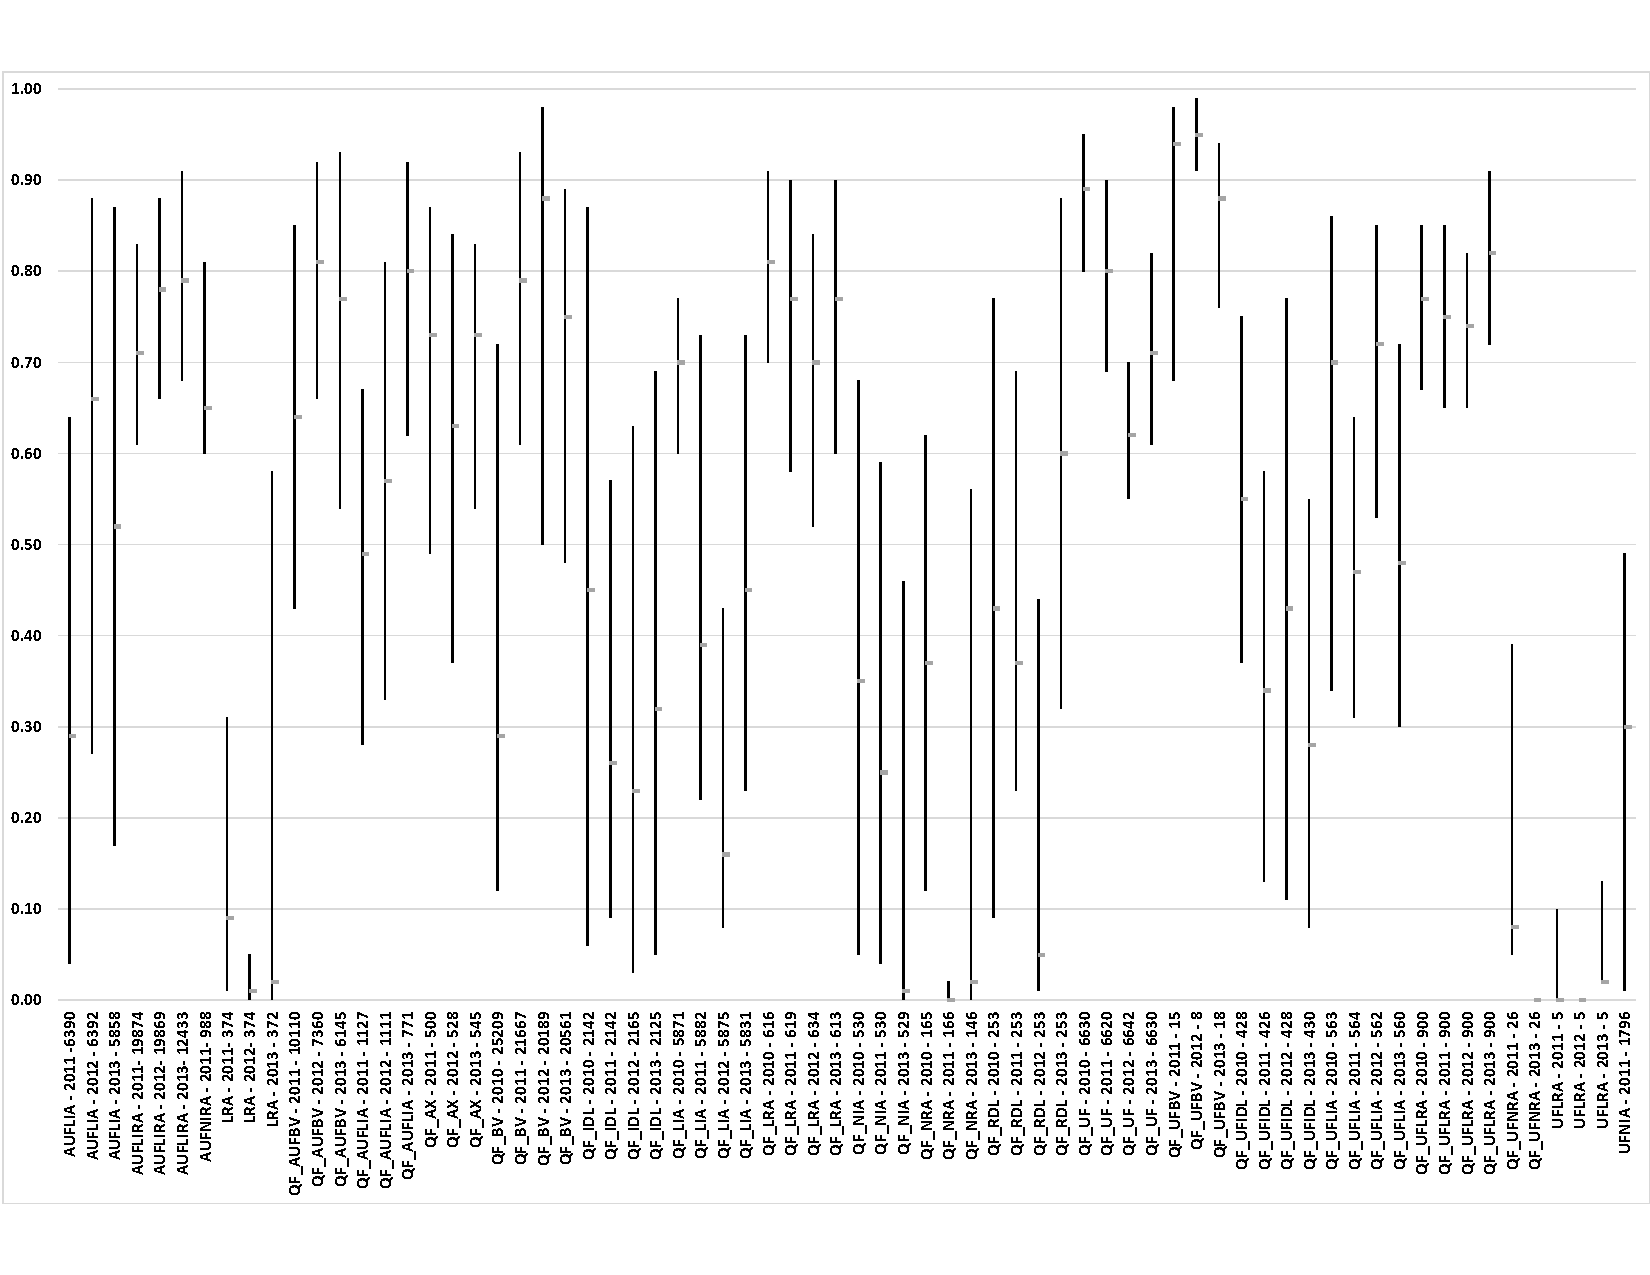
\includegraphics[angle=270,origin=c,width=\columnwidth,height=1.5\columnwidth]{runnerup.pdf}
\caption{Runner-up: Ratio of winning time to runner-up time, showing median, first and third quartiles.}
\label{Fig:runnerup1}
\end{figure}

\begin{figure}
\centering
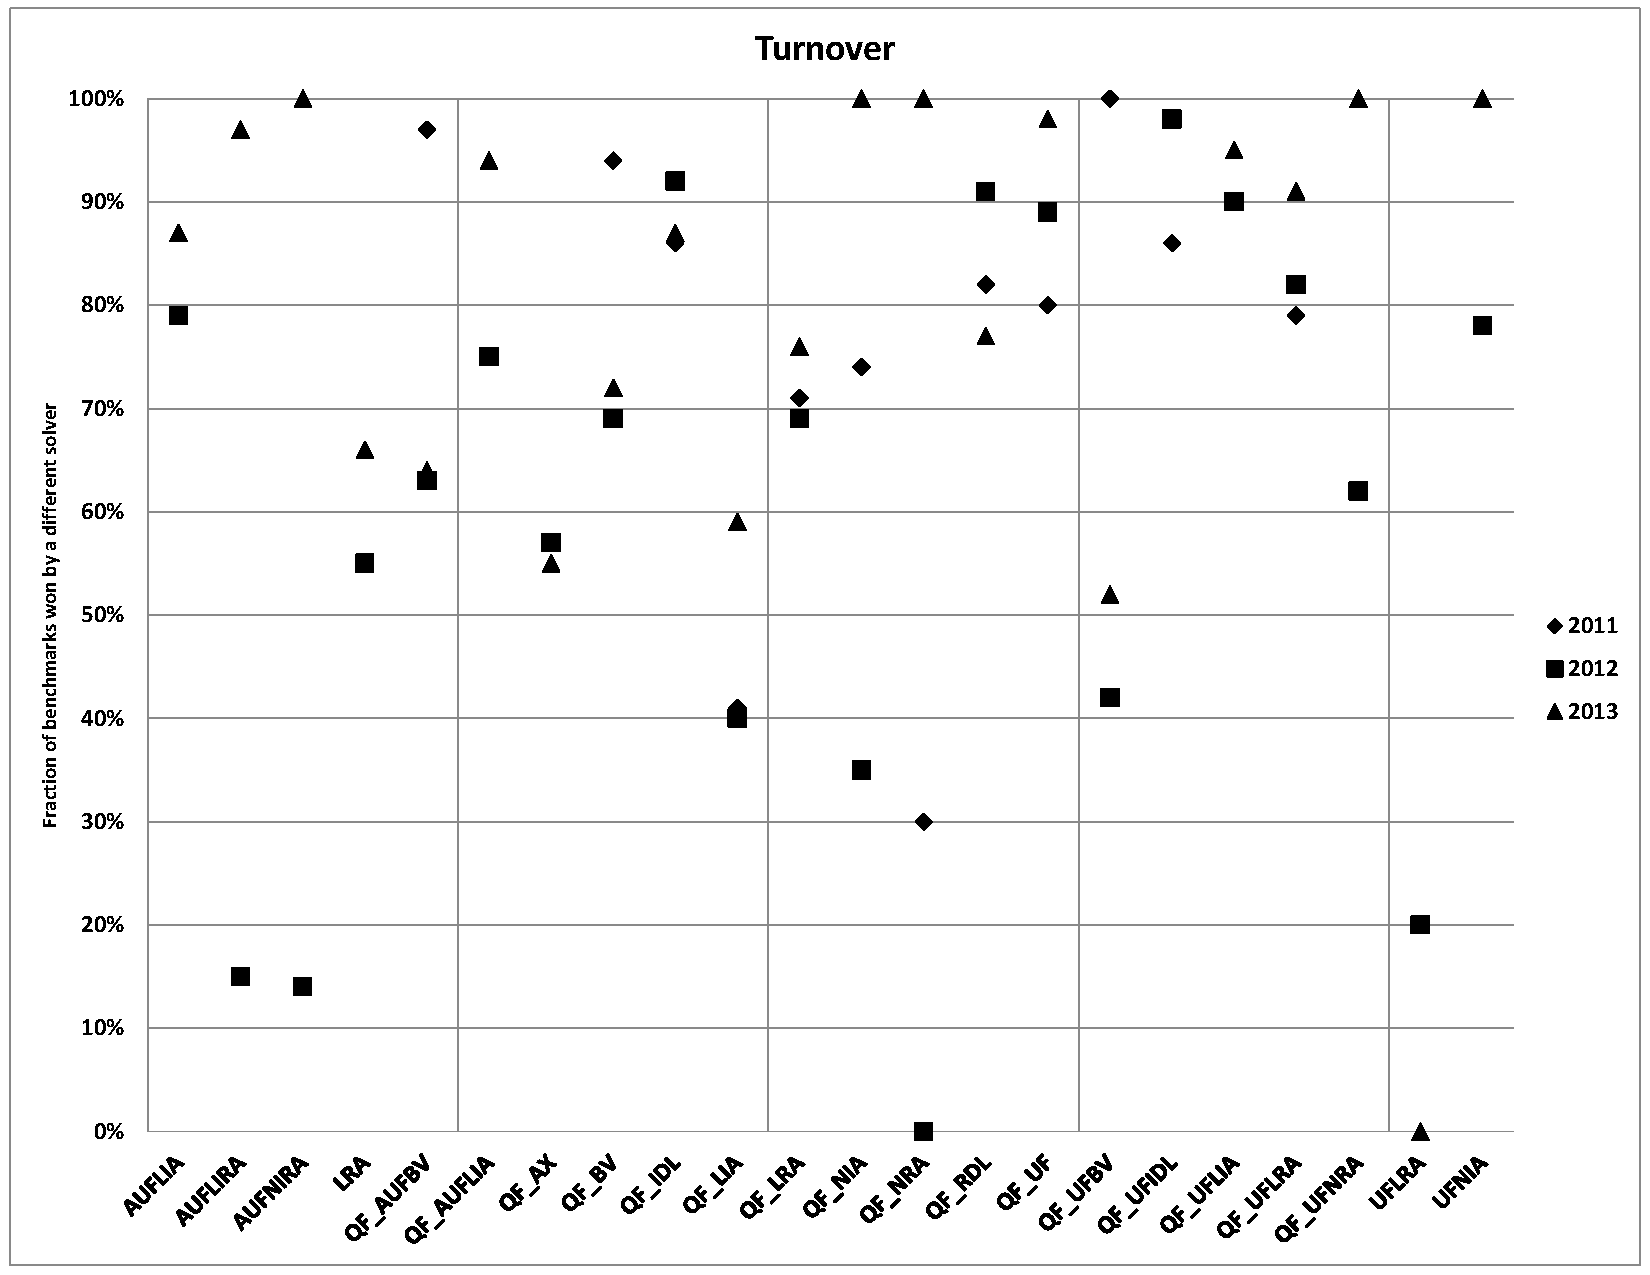
\includegraphics[width=\columnwidth]{turnover.pdf}
%\begin{tabular}{|l|rrr|p{.3in}|l|rrr|}
%\hline
%Logic & 2011 & 2012 & 2013 & & Logic & 2011 & 2012 & 2013 \\ \hline
AUFLIA & 0.79 & 0.79 & 0.87  & & QF\_NIA & 0.74 & 0.35 & 1.00 \\ 
AUFLIRA & 0.15 & 0.15 & 0.97 & & QF\_NRA & 0.30 & 0.00 & 1.00 \\  
AUFNIRA & 0.14 & 0.14 & 1.00 & & QF\_RDL & 0.82 & 0.91 & 0.77 \\ 
LRA & 0.55 & 0.55 & 0.66  & & QF\_UF & 0.80 & 0.89 & 0.98 \\  
QF\_AUFBV & 0.97 & 0.63 & 0.64 & & QF\_UFBV & 1.00 & 0.42 & 0.52 \\  
QF\_AUFLIA & 0.75 & 0.75 & 0.94 & & QF\_UFIDL & 0.86 & 0.98 & 0.98 \\  
QF\_AX & 0.57 & 0.57 & 0.55 & & QF\_UFLIA & 0.90 & 0.90 & 0.95 \\  
QF\_BV & 0.94 & 0.69 & 0.72 & & QF\_UFLRA & 0.79 & 0.82 & 0.91 \\  
QF\_IDL & 0.86 & 0.92 & 0.87 & & QF\_UFNRA & 0.62 & 0.62 & 1.00 \\  
QF\_LIA & 0.41 & 0.40 & 0.59 & & UFLRA & 0.20 & 0.20 & 0.00 \\  
QF\_LRA & 0.71 & 0.69 & 0.76 & & UFNIA & 0.78 & 0.78 & 1.00 \\  

%\hline
%\end{tabular}
\caption{Turnover: Fraction of benchmarks for the given year and logic for which the winning solver is from a different solver family than the prior year.}
\label{Fig:turnover}
\end{figure}


\begin{figure}
\centering
\centering
\begin{tabular}{|ll|ccrrr|}
\hline
Year & Logic & \# solvers & \# winners & winning dist., & scaled & \# benchmarks \\ \hline
2011 & AUFLIA & 2 & 2 & 1.36 & 0.68 & 6056 \\ \hline
2012 & AUFLIA & 2 & 2 & 1.61 & 0.81 & 5685 \\ \hline
2013 & AUFLIA & 3 & 3 & 1.69 & 0.56 & 5771 \\ \hline
2011 & AUFLIRA & 2 & 2 & 1.34 & 0.67 & 19791 \\ \hline
2012 & AUFLIRA & 2 & 2 & 1.42 & 0.71 & 19753 \\ \hline
2013 & AUFLIRA & 3 & 3 & 1.73 & 0.58 & 19845 \\ \hline
2011 & AUFNIRA & 2 & 2 & 1.32 & 0.66 & 987 \\ \hline
2011 & LRA & 2 & 2 & 1.58 & 0.79 & 322 \\ \hline
2012 & LRA & 2 & 2 & 1.02 & 0.51 & 358 \\ \hline
2013 & LRA & 2 & 2 & 1.52 & 0.76 & 344 \\ \hline
2011 & QF\_AUFBV & 5 & 5 & 2.16 & 0.43 & 14027 \\ \hline
2012 & QF\_AUFBV & 6 & 6 & 2.44 & 0.41 & 14124 \\ \hline
2013 & QF\_AUFBV & 5 & 5 & 2.55 & 0.51 & 14128 \\ \hline
2011 & QF\_AUFLIA & 3 & 3 & 1.60 & 0.53 & 1126 \\ \hline
2012 & QF\_AUFLIA & 3 & 3 & 2.01 & 0.67 & 1118 \\ \hline
2013 & QF\_AUFLIA & 4 & 4 & 1.84 & 0.46 & 1131 \\ \hline
2011 & QF\_AX & 4 & 4 & 2.27 & 0.57 & 547 \\ \hline
2012 & QF\_AX & 2 & 2 & 1.56 & 0.78 & 541 \\ \hline
2013 & QF\_AX & 3 & 3 & 1.87 & 0.62 & 548 \\ \hline
2010 & QF\_BV & 3 & 3 & 1.71 & 0.57 & 31094 \\ \hline
2011 & QF\_BV & 8 & 8 & 3.02 & 0.38 & 31320 \\ \hline
2012 & QF\_BV & 11 & 11 & 3.46 & 0.31 & 31369 \\ \hline
2013 & QF\_BV & 5 & 5 & 2.36 & 0.47 & 31230 \\ \hline
2010 & QF\_IDL & 3 & 3 & 1.87 & 0.62 & 1756 \\ \hline
2011 & QF\_IDL & 4 & 4 & 1.36 & 0.34 & 1954 \\ \hline
2012 & QF\_IDL & 2 & 2 & 1.15 & 0.57 & 1830 \\ \hline
2013 & QF\_IDL & 3 & 3 & 1.41 & 0.47 & 1956 \\ \hline
2010 & QF\_LIA & 3 & 3 & 1.45 & 0.48 & 5833 \\ \hline
2011 & QF\_LIA & 4 & 4 & 1.83 & 0.46 & 5829 \\ \hline
2012 & QF\_LIA & 4 & 4 & 1.44 & 0.36 & 5789 \\ \hline
2013 & QF\_LIA & 5 & 5 & 2.38 & 0.48 & 5859 \\ \hline
2010 & QF\_LRA & 5 & 5 & 2.10 & 0.42 & 618 \\ \hline
2011 & QF\_LRA & 6 & 6 & 2.42 & 0.40 & 620 \\ \hline
2012 & QF\_LRA & 4 & 4 & 1.63 & 0.41 & 619 \\ \hline
2013 & QF\_LRA & 5 & 5 & 2.42 & 0.48 & 627 \\ \hline

\end{tabular}
\caption{(Part 1) Winner distribution: The degree to which winning is distributed among solvers vs. dominated by one solver.}
\label{Fig:entropyA}
\end{figure}

\begin{figure}
\centering
\begin{tabular}{|ll|ccrrr|}
\hline
Logic & Year & \cellbr{\#\\Solvers} & \cellbr{\#\\Winners} & Winning dist., & scaled & \cellbr{\#\\Benchmarks} \\ \hline
QF\_NIA & 2010 & 3 & 3 & 1.64 & 0.55 & 530 \\
        & 2011 & 3 & 3 & 1.78 & 0.59 & 530 \\
        & 2013 & 2 & 2 & 1.58 & 0.79 & 526 \\ \hline
QF\_NRA & 2010 & 2 & 2 & 1.52 & 0.76 & 166 \\
        & 2011 & 2 & 1 & 1.00 & 0.50 & 166 \\
        & 2013 & 3 & 3 & 1.17 & 0.39 & 166 \\ \hline
QF\_RDL & 2010 & 3 & 3 & 1.61 & 0.54 & 220 \\
        & 2011 & 4 & 3 & 1.32 & 0.33 & 222 \\
        & 2012 & 2 & 2 & 1.04 & 0.52 & 213 \\
        & 2013 & 3 & 3 & 1.80 & 0.60 & 218 \\ \hline
QF\_UF & 2010 & 5 & 5 & 2.15 & 0.43 & 6643 \\
       & 2011 & 7 & 7 & 2.29 & 0.33 & 6647 \\
       & 2012 & 4 & 4 & 1.57 & 0.39 & 6643 \\
       & 2013 & 6 & 6 & 1.71 & 0.28 & 6647 \\ \hline
QF\_UFBV & 2011 & 4 & 2 & 1.59 & 0.40 & 31 \\
         & 2012 & 5 & 3 & 2.03 & 0.41 & 31 \\
         & 2013 & 5 & 3 & 1.75 & 0.35 & 31 \\ \hline
QF\_UFIDL & 2010 & 3 & 3 & 1.81 & 0.60 & 422 \\
          & 2011 & 4 & 4 & 1.43 & 0.36 & 423 \\
          & 2012 & 2 & 2 & 1.41 & 0.70 & 404 \\
          & 2013 & 3 & 3 & 1.32 & 0.44 & 423 \\ \hline
QF\_UFLIA & 2010 & 3 & 3 & 2.08 & 0.69 & 564 \\
          & 2011 & 4 & 4 & 1.41 & 0.35 & 564 \\
          & 2012 & 4 & 4 & 1.88 & 0.47 & 564 \\
          & 2013 & 5 & 4 & 1.70 & 0.34 & 564 \\ \hline
QF\_UFLRA & 2010 & 3 & 3 & 1.38 & 0.46 & 900 \\
          & 2011 & 4 & 2 & 1.43 & 0.36 & 900 \\
          & 2012 & 4 & 4 & 1.29 & 0.32 & 900 \\
          & 2013 & 5 & 4 & 1.95 & 0.39 & 900 \\ \hline
QF\_UFNRA & 2011 & 2 & 2 & 1.59 & 0.79 & 26 \\
          & 2013 & 2 & 1 & 1.00 & 0.50 & 26 \\ \hline
UFLRA & 2011 & 2 & 2 & 1.41 & 0.71 & 5 \\
      & 2012 & 2 & 1 & 1.00 & 0.50 & 5 \\
      & 2013 & 3 & 1 & 1.00 & 0.33 & 5 \\ \hline
UFNIA & 2011 & 2 & 2 & 1.41 & 0.71 & 1732 \\ \hline

\end{tabular}
\caption{(Part 2) Winner distribution: The degree to which winning is distributed among solvers vs. dominated by one solver.}
\label{Fig:entropyB}
\end{figure}


\begin{figure}
\centering
\begin{tabular}{|l|rrr|}
\hline
Solver & Total SOTAC & Mean over & Mean over \\ 
  &  & all attempted & all solved  \\ \hline
MiniSMT-0.5-SMT-EVAL-2013 & 397.00 & 0.57 & 0.60 \\ 
OpenSMT-SMT-EVAL-2013 & 1083.43 & 0.16 & 0.17 \\ 
SMTInterpol-2.0r8402-SMT-EVAL-2013 & 2829.63 & 0.19 & 0.20 \\ 
SONOLAR-2013-05-15-SMT-EVAL-2013 & 9031.47 & 0.20 & 0.21 \\ 
Boolector-1.5.118-SMT-EVAL-2013 & 9352.38 & 0.20 & 0.21 \\ 
veriT-SMT-EVAL-2013 & 11446.57 & 0.25 & 0.30 \\ 
MathSAT5-5.2.6-SMT-EVAL-2013 & 12285.92 & 0.20 & 0.21 \\ 
CVC4-SMT-EVAL-2013 & 21562.27 & 0.23 & 0.25 \\ 
Z3-4.3.2.a054b099c1d6-x64-debian-6.0.6-... & 25664.33 & 0.27 & 0.28 \\ 

\hline
\end{tabular}
\caption{State of the art contribution from each of the 2013 solvers, sorted by Total SOTAC.}
\label{Fig:sotac}
\end{figure}

\subsection{Sequential vs. parallel computation}
\label{parallel}

The StarExec cluster contains computation nodes with 4 cores each; solvers configured for multi-threaded computation can take advantage of the parallel processing possibilities and reduce their overall wall-clock time in solving a benchmark. Previous competitions have had demonstration divisions featuring parallel computation.
For this evaluation we set a wall-clock timeout of 25 minutes and a CPU-time timeout of 100 minutes. Thus the evaluation measured the performance of solvers for parallel computation, if they were so configured. A competition focused on sequential processing would set the wall-clock and CPU-time timeouts at the same value.
We did not rerun the evaluation data to assess sequential processing performance. The data showing both wall-clock and CPU time was not available when we did our 
primary evaluation, and some of the early CPU-time data appears inconsistent with the wall-clock times. Thus we left questions about parallel vs. sequential performance for further study: 
\begin{itemize}
\item what fraction of solvers use parallel computation?
\item what is the speedup generally achieved by these solvers and the kinds of problems represented by the benchmark set?
\item what is the observed overhead, that is, for purely sequential performance by how much does the wall-clock time exceed the CPU-time?
\item are competition results significantly different when judged by CPU time vs. wall-clock time?
\end{itemize}
We expect that the 2014 competition will generate a data set better able to answer these questions.

With respect to this study, note that we used solvers as they were historically configured. They may have been configured solely for sequential performance, and the authors do not know in every case what the configurations of the older solvers are. Modern configurations of the same solvers might make use of multiple cores. The configuration of StarExec used for the evaluation (4 cores, 25 minute timeout), might be less than ideal from some historical solvers, but it is typical of what a user might use at the present time. Thus, to repeat a point made elsewhere in this report, the results of the virtual competitions should not be used to compare specific solvers. Rather, they offer a comparison of different modes of organizing and running the competition.

\subsection{Benchmarks}
\label{Benchmarks}

The number of benchmarks has successfully grown since SMT-LIB was established; at the time of this evaluation, there were more than 100,000 in all of the logics combined, including both incremental and non-incremental collections. However, the logics differ significantly in the number of available benchmarks and in their overall difficulty.

SMT-LIB distinguishes four loosely-defined kinds of benchmarks:
\begin{itemize}[noitemsep,nolistsep]
\item {\em check} benchmarks are simple tasks that are designed to ensure that a solver has the basic functionality required for a division;
\item {\em industrial} benchmarks are generated from some application; ideally these are substantial examples showing real-world variation, but they may be from toy applications running on a toy examples;
\item {\em crafted} benchmarks are hand-crafted to exercise a particular bit of functionality or technical challenge
\item {\em random} benchmarks are randomly generated from some distribution.
\end{itemize}
Fig.~\ref{Fig:category} shows the number of benchmarks for each logic and the distribution over the categories just listed. The numbers vary considerably. Some logics, such as UFLRA, have just a very few benchmarks, while others have tens of thousands. Note that in nearly all logics, the bulk of the benchmarks are 
considered industrial.

The same table also shows the distribution of benchmarks among those known to be satisfiable, unsatisfiable, and with an unknown status. Here there is 
considerable variation. Some logics have nearly no satisfiable benchmarks. Some have a large proportion (at least as of 2013) of benchmarks of unknown status.
This is particularly the case for the popular and important QF\_BV logic.
Part of the effort of benchmark curation for the 2014 competition is to more carefully assign benchmarks to logics and to determine status that is currently unknown.

\begin{figure}
\centering
\begin{tabular}{|l|r|p{.45in}p{.3in}p{.35in}p{.25in}|p{.25in}p{.25in}p{.4in}|}
\hline
Logic & total & industrial & crafted & random & check & sat & unsat & unknown \\ \hline
AUFLIA & 6402 & 6375 & 26 & 0 & 128 & 9 & 4149 & 2244 \\ \hline
AUFLIRA & 19917 & 19717 & 200 & 0 & 0 & 100 & 19742 & 75 \\ \hline
AUFNIRA & 989 & 989 & 0 & 0 & 0 & 0 & 943 & 46 \\ \hline
LRA & 374 & 144 & 0 & 230 & 0 & 0 & 0 & 374 \\ \hline
QF\_AUFBV & 14335 & 14008 & 325 & 0 & 16 & 4795 & 3566 & 5974 \\ \hline
QF\_AUFLIA & 1140 & 114 & 1020 & 0 & 6 & 548 & 592 & 0 \\ \hline
QF\_AX & 551 & 0 & 551 & 0 & 0 & 272 & 279 & 0 \\ \hline
QF\_BV & 31748 & 29887 & 1160 & 3 & 10 & 2259 & 1378 & 28111 \\ \hline
QF\_IDL & 2170 & 628 & 980 & 63 & 2 & 942 & 691 & 537 \\ \hline
QF\_LIA & 5882 & 3832 & 737 & 1075 & 1118 & 2227 & 2584 & 1071 \\ \hline
QF\_LRA & 634 & 632 & 0 & 0 & 2 & 226 & 317 & 91 \\ \hline
QF\_NIA & 530 & 177 & 167 & 0 & 0 & 242 & 63 & 225 \\ \hline
QF\_NRA & 166 & 151 & 15 & 0 & 0 & 56 & 4 & 106 \\ \hline
QF\_RDL & 255 & 147 & 106 & 0 & 2 & 57 & 113 & 85 \\ \hline
QF\_UF & 6647 & 0 & 6647 & 0 & 0 & 2549 & 4094 & 4 \\ \hline
QF\_UFBV & 31 & 31 & 0 & 0 & 0 & 0 & 31 & 0 \\ \hline
QF\_UFIDL & 430 & 396 & 32 & 0 & 2 & 110 & 318 & 2 \\ \hline
QF\_UFLIA & 564 & 331 & 231 & 0 & 2 & 396 & 168 & 0 \\ \hline
QF\_UFLRA & 900 & 0 & 0 & 900 & 0 & 409 & 407 & 84 \\ \hline
QF\_UFNRA & 26 & 26 & 0 & 0 & 0 & 15 & 0 & 11 \\ \hline
UFLRA & 5 & 0 & 5 & 0 & 0 & 5 & 0 & 0 \\ \hline
UFNIA & 1796 & 1796 & 0 & 0 & 0 & 0 & 1660 & 136 \\ \hline
TOTAL & 95492 & 79381 & 12202 & 2271 & 1288 & 15217 & 41099 & 39176 \\ \hline

\end{tabular}
\caption{The numbers of benchmarks by logic, category, and result.}
\label{Fig:category}
\end{figure}

Some benchmarks are {\em incremental}; that is, they contain more than one {\tt check-sat} command in a command script. This is relevant to interactive applications, but is not the main focus of the competition. In 2012, there were demonstration divisions on generating unsat cores and proof generation. These did not require special benchmarks, but do require different evaluation. The evaluation reported here did not consider the incremental benchmarks.


Fig.~\ref{Fig:completion} shows the fraction of benchmarks (for each logic and year) that are solved within the 25 minute timeout period. For each combination of solver and year we report the fraction of benchmarks that are completed by all solvers and the fraction that are completed by at least one solver. In 2013, in about half of the logics, all benchmarks are completed by at least one solver within the timeout period (though not necessarily the same solver); in all but one logic (QF\_RDL), at least 95\% of the benchmarks are completed by at least one solver. The values for the fraction of benchmarks completed by all solvers are not as high, since some of the solvers may be initial experimental versions and not tuned for competition. Even so, in more than half of the logics, at least 85\% of benchmarks were completed by all solvers.

Fig.~\ref{Fig:quintiles} is another view of benchmark difficulty. Here, for each logic, the distributions of winning times among the 2013 solvers are shown. In particular, selected
percentiles of each distribution are tabulated (the value for the {\em n}th percentile is the number of seconds for which that fraction of the benchmarks is completed by the winning solver for that benchmark). In all but three logics more than 80\% of the benchmarks for that logic take less than just a few seconds, if not less than a second. Only four of the logics have more than 5\% of their benchmarks that take more than the timeout period.
 
These results indicate that there is substantial room for more difficult benchmarks in almost all of the logics. On the other hand, if the benchmarks are indeed typical of application problems, the results indicate that today's solvers are very capable.

An additional question that would be interesting to address in a benchmark evaluation
 is the degree to which benchmarks discriminate among solvers. A small set of `discriminating' benchmarks would be more useful than a large set of undifferentiated ones. One could, for example, measure a quantity akin to the SOTAC measure of section \ref{Competitiveness}: benchmarks that are easy for all solvers would be discounted, ones that are hard for all would be challenges, and ones that show a wide range of performance might be discriminating benchmarks.

For example, consider a competition with just two solvers. There are then four categories of benchmarks corresponding to the subsets of solvers that solve the
benchmarks. The key point is whether benchmarks that are grouped together would nearly always be grouped together in other competitions with other sets of solvers or other competition rules. To fully elucidate this question will require analysis of the characteristics of the benchmarks combined with 
experimental assessment of their similarity in a wide variety of competition designs. We determined that the principal data collection of SMT-EVAL was not adequate to answer this question and that it deserved a full analysis in 
conjunction with a broad evaluation of benchmarks.

\begin{figure}
\centering
\begin{tabular}{|l|r|rrrr|rrrr|}
\hline
Logic & \parbox[t]{.7in}{\# \\ Benchmarks} & \parbox[t]{.3in}{2010 \\ all} & \parbox[t]{.3in}{2011 \\ all} & \parbox[t]{.3in}{2012 \\ all} & \parbox[t]{.3in}{2013 \\ all} & \parbox[t]{.3in}{2010 \\ any} & \parbox[t]{.3in}{2011 \\ any} & \parbox[t]{.3in}{2012 \\ any} & \parbox[t]{.3in}{2013 \\ any} \\ \hline
AUFLIA & 6402
 & 0.80 & 0.75 & 0.73 & 0.65 & 0.80 & 0.95 & 0.89 & 0.90 \\
AUFLIRA & 19917
 & 0.98 & 0.97 & 0.95 & 0.94 & 0.98 & 0.99 & 0.99 & 1.00 \\
AUFNIRA & 989
 & 0.98 & 0.98 & 0.99 & 0.99 & 0.98 & 1.00 & 0.99 & 0.99 \\
LRA & 374
 & 0.78 & 0.57 & 0.73 & 0.56 & 0.78 & 0.86 & 0.96 & 0.92 \\
QF\_AUFBV & 14335
 & 0.85 & 0.79 & 0.80 & 0.89 & 0.85 & 0.98 & 0.99 & 0.99 \\
QF\_AUFLIA & 1140
 & 0.93 & 0.86 & 0.85 & 0.89 & 0.93 & 0.99 & 0.98 & 0.99 \\
QF\_AX & 551
 & 0.94 & 0.86 & 0.90 & 0.89 & 0.94 & 0.99 & 0.98 & 0.99 \\
QF\_BV & 31747
 & 0.87 & 0.84 & 0.82 & 0.91 & 0.98 & 0.99 & 0.99 & 0.98 \\
QF\_IDL & 2170
 & 0.44 & 0.47 & 0.50 & 0.65 & 0.81 & 0.90 & 0.84 & 0.90 \\
QF\_LIA & 5882
 & 0.80 & 0.24 & 0.33 & 0.35 & 0.99 & 0.99 & 0.98 & 1.00 \\
QF\_LRA & 634
 & 0.74 & 0.73 & 0.73 & 0.92 & 0.97 & 0.98 & 0.98 & 0.99 \\
QF\_NIA & 530
 & 0.78 & 0.56 & 0.98 & 0.67 & 1.00 & 1.00 & 0.98 & 0.99 \\
QF\_NRA & 166
 & 0.93 & 0.46 & 1.00 & 0.52 & 1.00 & 1.00 & 1.00 & 1.00 \\
QF\_RDL & 255
 & 0.52 & 0.51 & 0.52 & 0.80 & 0.86 & 0.87 & 0.84 & 0.85 \\
QF\_UF & 6647
 & 0.96 & 0.95 & 0.96 & 0.95 & 1.00 & 1.00 & 1.00 & 1.00 \\
QF\_UFBV & 31
 & 1.00 & 0.26 & 0.42 & 0.39 & 1.00 & 1.00 & 1.00 & 1.00 \\
QF\_UFIDL & 430
 & 0.73 & 0.73 & 0.72 & 0.89 & 0.98 & 0.98 & 0.94 & 0.98 \\
QF\_UFLIA & 564
 & 0.91 & 0.91 & 0.91 & 0.88 & 1.00 & 1.00 & 1.00 & 1.00 \\
QF\_UFLRA & 900
 & 0.89 & 0.61 & 0.61 & 1.00 & 1.00 & 1.00 & 1.00 & 1.00 \\
QF\_UFNRA & 26
 & 1.00 & 0.96 & 1.00 & 0.85 & 1.00 & 1.00 & 1.00 & 1.00 \\
UFLRA & 5
 & 1.00 & 0.60 & 0.40 & 0.20 & 1.00 & 1.00 & 1.00 & 1.00 \\
UFNIA & 1796
 & 0.63 & 0.74 & 0.74 & 0.96 & 0.63 & 0.96 & 0.74 & 0.96 \\ \hline

\end{tabular}
\caption{The fraction of benchmarks completed by the solvers for the given year and logic.}
\label{Fig:completion}
\end{figure}

\begin{figure}
\centering
\begin{tabular}{|l|r|rrrr|}
\hline
Logic & \# & Median & 80th percentile & 90th percentile & 95th percentile  \\ \hline
AUFLIA & 6402 & 0.02 & 0.07 & 7.26 & 1600.00 \\ 
AUFLIRA & 19917 & 0.01 & 0.01 & 0.01 & 0.02 \\ 
AUFNIRA & 989 & 0.01 & 0.01 & 0.02 & 0.02 \\ 
LRA & 374 & 0.02 & 0.07 & 2.81 & 1600.00 \\ 
QF\_AUFBV & 14335 & 0.01 & 0.02 & 0.05 & 0.16 \\ 
QF\_AUFLIA & 1140 & 0.01 & 0.01 & 0.02 & 0.04 \\ 
QF\_AX & 551 & 0.02 & 0.03 & 0.05 & 0.07 \\ 
QF\_BV & 31747 & 0.01 & 0.15 & 0.58 & 1.06 \\ 
QF\_IDL & 2170 & 0.74 & 28.61 & 1355.54 & 1600.00 \\ 
QF\_LIA & 5882 & 0.30 & 3.91 & 11.97 & 19.02 \\ 
QF\_LRA & 634 & 0.09 & 1.12 & 8.89 & 25.38 \\ 
QF\_NIA & 530 & 0.02 & 0.15 & 0.69 & 1.61 \\ 
QF\_NRA & 166 & 0.01 & 0.01 & 0.01 & 0.01 \\ 
QF\_RDL & 255 & 1.76 & 41.93 & 1600.00 & 1600.00 \\ 
QF\_UF & 6647 & 0.03 & 0.12 & 0.28 & 0.48 \\ 
QF\_UFBV & 31 & 0.01 & 0.01 & 0.01 & 0.01 \\ 
QF\_UFIDL & 430 & 0.13 & 0.67 & 2.28 & 15.11 \\ 
QF\_UFLIA & 564 & 0.02 & 0.03 & 0.05 & 0.10 \\ 
QF\_UFLRA & 900 & 0.03 & 0.04 & 0.05 & 0.06 \\ 
QF\_UFNRA & 26 & 0.01 & 0.01 & 0.01 & 0.01 \\ 
UFLRA & 5 & 3.30 & 28.19 & 28.19 & 28.19 \\ 
UFNIA & 1796 & 0.22 & 2.40 & 59.47 & 383.20 \\ 

\hline
\end{tabular}
\caption{The distribution of winning benchmark times by logic (for 2013 solvers).}
\label{Fig:quintiles}
\end{figure}

\subsection{Application needs}
\label{Applications}

As part of its evaluation, the SMT-EVAL team solicited input on applications that use SMT-LIB. The response was not broad enough to be representative. In addition, the authors 
have encountered, by happenstance, enough users of SMT-LIB who are not active in the user community to indicate that there is likely a wide variety of uses that are not well-organized or well-represented in benchmarks on specific logics. A few application domains are fairly well-known, including software verification and synthesis, scheduling, planning and routing optimization, and invariant inference. Software verification applications in particular will benefit from broader support for combinations of theories and better heuristics for quantification. 

In general, a better understanding of the variety of application needs is needed to target future development of SMT solvers and the SMT benchmark library.

%{\em Scheduling problems} typically use difference logics, either integer or real. A recent example is the Mihal's paper \cite{Mihal2013} at the SMT 2013 workshop.
%
%
%{\em Software verification} research uses SMT solvers to discharge verification conditions. In a purely model checking formalism, without user supplied axioms and specifications, a {\tt QF\_BV} or {\tt QF\_UFBV} logic would be sufficient (the latter is not defined, but would seem straightforward). However, in the formalism used by tools such as OpenJML \cite{Cok-2014-OpenJML,Cok-2011-OpenJML}, Dafny \cite{Leino:Dafny:LPAR16,Dafny2014} or Frama-C \cite{webframac}, both code and user-supplied specifications are translated to a logical form, expressed in SMT-LIB. In this case, the logic requires a broad range of underlying theories, including quantification. For this purpose solvers need to support all of the characteristics listed in subsection \ref{Lattice} and add support (theories and decision procedures) for strings, partially-ordered sets (to represent programming language types), and innovative theories and decision procedures to reason about uses of dynamic memory. Similarly SMT solvers are used underneath Ada tools 
%
%{\em Function synthesis}. A newer application of SMT constraint solving is to find functions or predicates satisfying given properties. Heizmann and Leike \cite{webLasso}
%use QF\_LRA and QF\_NRA logics to synthesize appropriate ranking functions for loops. 
%Similar work by the same authors uses interpolants to create or refine specifications; thus they use the interpolant-generation capability of some SMT solvers and the QF\_UFLIRA or AUFNIRA logics.

\section{Conclusions and recommendations}
\label{Conclusions}

\subsection{Observations from the evaluation data}

The analyses described point to three principal conclusions and a number of observations.
\begin{itemize}
\item First, unsurprisingly, there is still a need for more and better benchmarks, despite the successful growth and current large quantity ($>$ 100,000) of benchmarks in SMT-LIB. Some logics have few benchmarks. In most logics, only a small fraction of benchmarks are significantly challenging (measured by time required to solve them).
Effort toward determining status of benchmarks whose status is currently unknown would also be worthwhile.
\item Related to the above, a better sense of the application areas of SMT is needed. Such an analysis will drive solver research in application-oriented directions, provide focus on application-oriented logics, and guide application-relevant benchmark acquisition.
\item Finally, we discovered that using a random subset of benchmarks as the basis for the annual competition, together with inherent non-determinism in running solvers, significantly lessens the ability of a competition to determine `best' solvers at a given point in time. Simply rerunning a competition is quite likely to result in a different ordering of results. The best mitigation is to run as large a benchmark set as possible in a competition (and to work toward application-relevant benchmark sets).
\end{itemize}

Other observations are these:
\begin{itemize}
\item {\em Participation}. The number of participants is relatively stable (9-13) with an average turnover of 35\% (low of 16\%, high of 50\%) each year. There is also a core of continuing participants (about 1/3 of the total).
\item {\em Progress in solver performance}. Solver performance increased significantly from 2010 to 2013. 
Most of that improvement occurred from 2010 to 2011; we did not determine a reason for that improvement. There is improvement across nearly all logics, though some logics are lagging.  
\item {\em Repeatability}. The repeatability of benchmarks is reduced by solver nondeterminism. Most importantly, however, competition repeatability is compromised by significant differences in performance of solvers on particular benchmarks, such that different random subsets of benchmarks will produce different assessments of solvers. The relevance of competitions is also threatened by the relevance of the total benchmark set.
\item {\em Competitiveness of solvers}. Within a logic nearly all solvers contribute something (e.g., a solution that no other solver produces). However, generally the winning times across benchmarks within a logic are obtained by 2-3 solvers that dominate that division. Comparing first-place times to second-place times shows that (a) in many logics the runner-up is quite close to the winner, but (b) in some logics, presumably with state-of-the-art tuning and advanced algorithms, the winner far outstrips the other competitors. It is also relevant that most benchmarks change winner from one year to the next. Overall, we judge that there is a moderate degree of competitiveness among solvers - a few tend to dominate in any logic, but other solvers do also make their contribution.
\item {\em Difficulty of Benchmarks}. A relatively low fraction of benchmarks require more than the timeout period to solve. Most benchmarks are solved by all solvers within the timeout period.

\end{itemize}

\subsection{Recommendations for competitions and for SMT-LIB}

The experience of past competitions and this evaluation point to a number of ideas for future competitions. Most past policies have worked well and should be continued: openness, transparency, reproducibility, public submission of solvers. Other aspects could use improvement. Some of these have already begun for 2014.
\begin{itemize}
\item To reduce potential variation caused by choice of benchmarks in a competition, a competition should include as many benchmarks as possible.
\item Invigorate the collection of benchmarks and promote a round of curating the existing benchmarks. This might include discontinuing or combining some logics.
\item Encourage the participation of new entrants through tool support and recognition. Some ideas are recognizing the best new entrant and promoting reference infrastructure for elements like parsing input files or standard reporting mechanisms.
\item Encourage broad participation by measuring performance in all logics, even when some logics are deemed more relevant than others.
\item Encourage broadening measures of performance beyond solution of single satisfiability problems, by including, for example, determining unsat cores, measuring performance on incremental benchmarks, computing interpolants, producing proofs, producing satisfying assignments, or encouraging solvers that use multi-processing implementations.
\item Investigate the naming convention and inclusion relationships for logics, with the goal of simplifying the relationships and with an eye toward adding additional theories and a significant expansion of the number of logics. This may not mean changing existing names, but would at least set a policy for how new theories and logics are to be named. At minimum this would clarify the process of naming new theories and logics.
\item There is a relative paucity of difficult benchmarks (those that are not solved within the timeout period). Perhaps this is because of progress in solver performance and in hardware speed. In either case, additional difficult benchmarks are needed.
\item The scoring criterion should be revisited. The current scoring emphasizes number solved over time to solve. First, time performance is important to applications, perhaps even more than solving the last 10\% of hard problems, so some balance between number solved and time to solve might be appropriate. Second, some solvers issue `unknown' indicating a possible satisfying solution is available, but it is not known to be sound (perhaps because of the presence of quantifiers). Such a solution may be available well before a timeout; however, such a result currently counts the same as a timeout.
\end{itemize}

\subsection{Future work}
The most important aspect of future work is to increase and improve benchmark quality, as described above. Thus we would encourage
\begin{itemize}
\item a broad survey of SMT application domains and their needs in solver support, both logics and functionality beyond determining satisfiability. 
A corresponding review of the benchmarks in SMT-LIB would determine the degree
to which benchmarks are representative of the application domains and would 
provide guidelines for collecting new benchmarks.
\end{itemize}
There are also a number of questions that we posed but did not have the time or data to answer. 
\begin{itemize}
\item Are there interesting differences in performance between satisfiable and unsatisfiable benchmarks?
\item Do solvers support all of SMT-LIB~v2? Should the community encourage expansion to new capabilities (e.g., unsat cores, incremental, interpolants, model generation, proof generation)? Should the community define a core language that is used for the competition, with other aspects being optional?
\item Which logics should be retired or deemphasized, based on solver progress or application need?
\item Competitions primarily measure ability to solve benchmarks, with the time to do so a secondary criterion. However, in some applications it is important to discharge easy problems quickly. We did not assess this characteristic of the available solvers, but it would be worth doing so.
\item It would also be worth extending our study with an evaluation of incremental benchmarks and means of measuring performance in an interactive environment.
\item Measuring the contribution of individual benchmarks.
\end{itemize}

As this report is being finalized, the 2014 SMT Competition is underway. Some of the proposals and hopes expressed in this report have been realized: 2014 is seeing a record number of participants, including new solver entries; there is a record number of benchmarks being used; and with only minor, recoverable problems, the StarExec infrastructure is performing a massive amount of computation over a week or so of competition time.


%\section*{Acknowledgments} 
\begin{acknowledgements} 
 
The cost of executing the SMT competition is underwritten by the SMT
Workshop.  The evaluation used the Star-Exec cluster at the University
of Iowa.  This computation cluster replaces the SMT-Exec cluster used
for all previous competitions.  The cluster is supported by the
U.S.\ National Science Foundation under grants \#1058748 and \#1058925.  Cok's
contribution is supported by GrammaTech, Inc.\ and in part by the
National Science Foundation under grant ACI-1314674.  Any opinions,
findings, and conclusions or recommendations expressed in this
material are those of the authors and do not necessarily reflect the
views of the National Science Foundation.
\end{acknowledgements}
 
\bibliographystyle{plain}
\bibliography{SMTEVAL-2013,cok,sv}

\end{document}
